% Options for packages loaded elsewhere
\PassOptionsToPackage{unicode}{hyperref}
\PassOptionsToPackage{hyphens}{url}
\PassOptionsToPackage{dvipsnames,svgnames,x11names}{xcolor}
%
\documentclass[
  letterpaper,
  DIV=11,
  numbers=noendperiod]{scrartcl}

\usepackage{amsmath,amssymb}
\usepackage{iftex}
\ifPDFTeX
  \usepackage[T1]{fontenc}
  \usepackage[utf8]{inputenc}
  \usepackage{textcomp} % provide euro and other symbols
\else % if luatex or xetex
  \usepackage{unicode-math}
  \defaultfontfeatures{Scale=MatchLowercase}
  \defaultfontfeatures[\rmfamily]{Ligatures=TeX,Scale=1}
\fi
\usepackage{lmodern}
\ifPDFTeX\else  
    % xetex/luatex font selection
\fi
% Use upquote if available, for straight quotes in verbatim environments
\IfFileExists{upquote.sty}{\usepackage{upquote}}{}
\IfFileExists{microtype.sty}{% use microtype if available
  \usepackage[]{microtype}
  \UseMicrotypeSet[protrusion]{basicmath} % disable protrusion for tt fonts
}{}
\makeatletter
\@ifundefined{KOMAClassName}{% if non-KOMA class
  \IfFileExists{parskip.sty}{%
    \usepackage{parskip}
  }{% else
    \setlength{\parindent}{0pt}
    \setlength{\parskip}{6pt plus 2pt minus 1pt}}
}{% if KOMA class
  \KOMAoptions{parskip=half}}
\makeatother
\usepackage{xcolor}
\setlength{\emergencystretch}{3em} % prevent overfull lines
\setcounter{secnumdepth}{5}
% Make \paragraph and \subparagraph free-standing
\ifx\paragraph\undefined\else
  \let\oldparagraph\paragraph
  \renewcommand{\paragraph}[1]{\oldparagraph{#1}\mbox{}}
\fi
\ifx\subparagraph\undefined\else
  \let\oldsubparagraph\subparagraph
  \renewcommand{\subparagraph}[1]{\oldsubparagraph{#1}\mbox{}}
\fi


\providecommand{\tightlist}{%
  \setlength{\itemsep}{0pt}\setlength{\parskip}{0pt}}\usepackage{longtable,booktabs,array}
\usepackage{calc} % for calculating minipage widths
% Correct order of tables after \paragraph or \subparagraph
\usepackage{etoolbox}
\makeatletter
\patchcmd\longtable{\par}{\if@noskipsec\mbox{}\fi\par}{}{}
\makeatother
% Allow footnotes in longtable head/foot
\IfFileExists{footnotehyper.sty}{\usepackage{footnotehyper}}{\usepackage{footnote}}
\makesavenoteenv{longtable}
\usepackage{graphicx}
\makeatletter
\def\maxwidth{\ifdim\Gin@nat@width>\linewidth\linewidth\else\Gin@nat@width\fi}
\def\maxheight{\ifdim\Gin@nat@height>\textheight\textheight\else\Gin@nat@height\fi}
\makeatother
% Scale images if necessary, so that they will not overflow the page
% margins by default, and it is still possible to overwrite the defaults
% using explicit options in \includegraphics[width, height, ...]{}
\setkeys{Gin}{width=\maxwidth,height=\maxheight,keepaspectratio}
% Set default figure placement to htbp
\makeatletter
\def\fps@figure{htbp}
\makeatother
% definitions for citeproc citations
\NewDocumentCommand\citeproctext{}{}
\NewDocumentCommand\citeproc{mm}{%
  \begingroup\def\citeproctext{#2}\cite{#1}\endgroup}
\makeatletter
 % allow citations to break across lines
 \let\@cite@ofmt\@firstofone
 % avoid brackets around text for \cite:
 \def\@biblabel#1{}
 \def\@cite#1#2{{#1\if@tempswa , #2\fi}}
\makeatother
\newlength{\cslhangindent}
\setlength{\cslhangindent}{1.5em}
\newlength{\csllabelwidth}
\setlength{\csllabelwidth}{3em}
\newenvironment{CSLReferences}[2] % #1 hanging-indent, #2 entry-spacing
 {\begin{list}{}{%
  \setlength{\itemindent}{0pt}
  \setlength{\leftmargin}{0pt}
  \setlength{\parsep}{0pt}
  % turn on hanging indent if param 1 is 1
  \ifodd #1
   \setlength{\leftmargin}{\cslhangindent}
   \setlength{\itemindent}{-1\cslhangindent}
  \fi
  % set entry spacing
  \setlength{\itemsep}{#2\baselineskip}}}
 {\end{list}}
\usepackage{calc}
\newcommand{\CSLBlock}[1]{\hfill\break\parbox[t]{\linewidth}{\strut\ignorespaces#1\strut}}
\newcommand{\CSLLeftMargin}[1]{\parbox[t]{\csllabelwidth}{\strut#1\strut}}
\newcommand{\CSLRightInline}[1]{\parbox[t]{\linewidth - \csllabelwidth}{\strut#1\strut}}
\newcommand{\CSLIndent}[1]{\hspace{\cslhangindent}#1}

\usepackage{booktabs}
\usepackage{longtable}
\usepackage{array}
\usepackage{multirow}
\usepackage{wrapfig}
\usepackage{float}
\usepackage{colortbl}
\usepackage{pdflscape}
\usepackage{tabu}
\usepackage{threeparttable}
\usepackage{threeparttablex}
\usepackage[normalem]{ulem}
\usepackage{makecell}
\usepackage{xcolor}
\usepackage{tabularray}
\usepackage[normalem]{ulem}
\usepackage{graphicx}
\UseTblrLibrary{booktabs}
\UseTblrLibrary{rotating}
\UseTblrLibrary{siunitx}
\NewTableCommand{\tinytableDefineColor}[3]{\definecolor{#1}{#2}{#3}}
\newcommand{\tinytableTabularrayUnderline}[1]{\underline{#1}}
\newcommand{\tinytableTabularrayStrikeout}[1]{\sout{#1}}
\KOMAoption{captions}{tableheading}
\makeatletter
\@ifpackageloaded{caption}{}{\usepackage{caption}}
\AtBeginDocument{%
\ifdefined\contentsname
  \renewcommand*\contentsname{Table of contents}
\else
  \newcommand\contentsname{Table of contents}
\fi
\ifdefined\listfigurename
  \renewcommand*\listfigurename{List of Figures}
\else
  \newcommand\listfigurename{List of Figures}
\fi
\ifdefined\listtablename
  \renewcommand*\listtablename{List of Tables}
\else
  \newcommand\listtablename{List of Tables}
\fi
\ifdefined\figurename
  \renewcommand*\figurename{Figure}
\else
  \newcommand\figurename{Figure}
\fi
\ifdefined\tablename
  \renewcommand*\tablename{Table}
\else
  \newcommand\tablename{Table}
\fi
}
\@ifpackageloaded{float}{}{\usepackage{float}}
\floatstyle{ruled}
\@ifundefined{c@chapter}{\newfloat{codelisting}{h}{lop}}{\newfloat{codelisting}{h}{lop}[chapter]}
\floatname{codelisting}{Listing}
\newcommand*\listoflistings{\listof{codelisting}{List of Listings}}
\makeatother
\makeatletter
\makeatother
\makeatletter
\@ifpackageloaded{caption}{}{\usepackage{caption}}
\@ifpackageloaded{subcaption}{}{\usepackage{subcaption}}
\makeatother
\ifLuaTeX
  \usepackage{selnolig}  % disable illegal ligatures
\fi
\usepackage{bookmark}

\IfFileExists{xurl.sty}{\usepackage{xurl}}{} % add URL line breaks if available
\urlstyle{same} % disable monospaced font for URLs
\hypersetup{
  pdftitle={Barriers to Green Living: Insights from 2018 and 2021 Toronto Climate Perception Surveys},
  pdfauthor={Lexi Knight},
  colorlinks=true,
  linkcolor={blue},
  filecolor={Maroon},
  citecolor={Blue},
  urlcolor={Blue},
  pdfcreator={LaTeX via pandoc}}

\title{Barriers to Green Living: Insights from 2018 and 2021 Toronto
Climate Perception Surveys\thanks{Code and data are available at:
\url{https://github.com/LexiKnight/toronto_climate/tree/main}.}}
\usepackage{etoolbox}
\makeatletter
\providecommand{\subtitle}[1]{% add subtitle to \maketitle
  \apptocmd{\@title}{\par {\large #1 \par}}{}{}
}
\makeatother
\subtitle{Uncovering What Stops Sustainable Behaviors and How
Communities Can Overcome Them}
\author{Lexi Knight}
\date{December 3, 2024}

\begin{document}
\maketitle
\begin{abstract}
This study examines the relationship between demographic factors---age,
education, and self-reported knowledge of climate change---and
individuals' likelihood of engaging in climate-friendly behaviors. The
analysis reveals that younger people and those with higher levels of
education are more likely to adopt sustainable actions such as reducing
car use and purchasing electric vehicles. However, the study also
highlights that financial barriers and limited access to resources
remain significant obstacles for broader climate action. These findings
underscore the importance of tailoring policies and interventions to
make sustainable behaviors more accessible to diverse demographic
groups, promoting wider participation in efforts to combat climate
change.
\end{abstract}

\renewcommand*\contentsname{Table of contents}
{
\hypersetup{linkcolor=}
\setcounter{tocdepth}{3}
\tableofcontents
}
\section{Introduction}\label{introduction}

Climate change is one of the most urgent challenges we face today. From
rising temperatures to extreme weather events, the planet is already
feeling the consequences of human-driven environmental change
(Intergovernmental Panel on Climate Change (IPCC) 2023). Yet, despite
widespread awareness of these risks, many people still struggle to adopt
behaviors that could help mitigate climate damage (Gifford 2011). This
gap between knowledge and action is a central puzzle that governments,
communities, and organizations are trying to solve (Kollmuss and Agyeman
2002). If we are to tackle this crisis effectively, we need to better
understand what stops people from acting, and how we can motivate change
(Steg 2014).

This paper examines how specific factors---such as age, education, and
self-reported knowledge of climate change---shape people's willingness
to engage in climate-friendly actions (Schultz 2002). By analyzing data
from a 2018 survey (City of Toronto 2024), we explore the connection
between demographic characteristics and behaviors like reducing energy
consumption, using greener transportation, and lowering waste. The
survey also delves into what prevents people from adopting these
behaviors, uncovering obstacles like cost, convenience, and skepticism
about the power of individual actions (Gifford 2011). With this
analysis, we aim to uncover how these factors interact and what they
mean for efforts to encourage sustainable choices (Stern 2000).

The heart of this study is to measure how age, education, and knowledge
of climate change influence the likelihood of adopting certain
behaviors. We found that younger individuals and those with higher
education levels are more likely to engage in actions like reducing car
usage and adopting plant-based diets (Fulton 2022). However, older
individuals are more inclined to take steps like cutting down on
household energy use (Lee 2019). Beyond these demographic trends, we
also discovered that barriers such as financial cost and doubts about
the effectiveness of individual efforts often hold people back from
taking action (Kollmuss and Agyeman 2002). These findings suggest that a
``one-size-fits-all'' approach to climate communication won't work.
Instead, targeted strategies that consider demographic differences are
essential for driving meaningful engagement (Steg 2014).

Understanding these patterns is crucial for crafting effective climate
policies. By identifying which groups are more likely to act and which
face significant barriers, we can better design interventions that speak
to people's concerns and motivations (Stern 2000). The implications of
this study go beyond simply knowing what people think about climate
change---they offer a roadmap for shaping messages and policies that
could shift behavior on a larger scale (Fulton 2022).

The remainder of this paper is structured as follows:
Section~\ref{sec-data} details the data and methods used in our
analysis. Section~\ref{sec-model} describes how we assess the factors
influencing climate-friendly behaviors across demographic groups.
\textbf{?@sec-results} highlights key differences in behavior based on
age, education, and knowledge of climate change.
\textbf{?@sec-discussion} discusses the findings, addresses the study's
limitations, and suggests directions for future research.
Section~\ref{sec-conclusion} concludes with a summary of the key
takeaways and actionable recommendations for enhancing climate action
engagement. Finally, Section~\ref{sec-appendix} contains supplementary
material.

\section{Data}\label{sec-data}

The primary data source for this project is the Climate Perception Study
dataset, provided by the City of Toronto via the Open Data Toronto
platform (City of Toronto 2024). This dataset offers insights into
public perceptions of climate change in Toronto and was accessed from
Open Data Toronto ({``Open Data Toronto''} 2024) on 6 November 2024.
\#\# Software and R-packages This project was conducted using the
statistical software \texttt{R} (R Core Team 2023). Data cleaning and
manipulation were primarily facilitated by the \texttt{tidyverse}
package (Wickham, Averick, et al. 2024), which encompasses various
essential tools. Within this suite, \texttt{dplyr} (Wickham, François,
et al. 2024) was employed for data manipulation tasks such as filtering,
summarizing, and joining datasets, while \texttt{readr} (Wickham,
Hester, et al. 2024) provided efficient functionality for reading and
writing rectangular text data. Specifically, the \texttt{write\_csv}
function from \texttt{tidyverse} was used to save the raw 2018 dataset.
To handle Excel files, we incorporated the \texttt{httr} package for
downloading files directly from online sources and \texttt{readxl}
(Wickham and Bryan 2024), which enabled us to read Excel files
seamlessly. Additionally, the \texttt{openxlsx} package was utilized to
create a new Excel workbook with multiple sheets, allowing us to store
the 2021 dataset in a structured format.

The \texttt{arrow} package was employed to handle large datasets
efficiently, ensuring smooth data processing, while \texttt{forcats} was
used for reordering factor levels to facilitate more insightful analyses
and visualizations. In terms of data tidying, the \texttt{tidyr} and
\texttt{stringr} packages allowed us to reshape and clean the data by
managing character strings and handling missing values. For the final
documentation and report generation, the \texttt{knitr} package was
instrumental in integrating R code and outputs into a cohesive and
reproducible report format. This suite of R packages collectively
enabled us to conduct thorough data management, manipulation, and
analysis, ultimately contributing to the successful completion of the
project.

\subsection{Methodology}\label{methodology}

\subsubsection{Data Collection}\label{data-collection}

The data for this analysis comes from two surveys commissioned by the
City of Toronto to assess residents' perceptions of climate change and
their willingness to take community action. In 2018, Environics Research
conducted n=404 online interviews with Toronto residents aged 18 and
older between October 11 and October 18. Each interview lasted
approximately 10 minutes. The sample was drawn from an online panel,
with quotas set by region, age, and gender to reflect the city's
population based on the 2016 Census, and minor weighting was applied.
Due to the non-random nature of the online survey, no margin of error
was assigned, though a random sample of this size would typically have a
margin of ±4.9 percentage points, 19 times out of 20.

In 2021, a second survey was conducted by Ipsos, a global market
research company. This survey included n=1,400 Toronto residents aged 18
and older and used a mixed-method approach. The sample consisted of
1,000 respondents from an online panel, 300 recruited via cell phone and
landline, and 100 online interviews conducted in Mandarin, Cantonese,
and Punjabi. This combination of methods aimed to enhance the survey's
representativeness. For analysis, Version 2 of the 2021 dataset, which
presents responses in a numeric format, was used.

\subsubsection{Data Analysis}\label{data-analysis}

The primary focus of this analysis was the 2018 dataset, examining six
key variables: age, education, extent informed, likelihood to take
action, reasons for not taking action, and the best method for
delivering information regarding climate change action. I analyzed these
variables at the individual level in the 2018 dataset by calculating the
percentages within each category, which provided a clear understanding
of the distribution and trends within the population.

In addition, I compared the 2018 dataset to the 2021 summary data to
assess changes over the years. By calculating the percentage
distribution for each variable in both years, I was able to identify any
shifts in public awareness, engagement, and preferences regarding
climate change action. This comparison revealed whether there have been
notable changes in factors like the public's level of information about
climate change, their likelihood to take action, and their preferred
communication methods.

This two-step approach allowed for a comprehensive understanding: a
detailed exploration of the 2018 data combined with a broader comparison
of trends between 2018 and 2021.

\subsection{Features}\label{features}

\subsubsection{Age}\label{age}

\paragraph{Individual 2018}\label{individual-2018}

Figure~\ref{fig-one} illustrates the age distribution of survey
respondents in 2018. The histogram displays the frequency of respondents
across different age groups, with the x-axis representing age intervals
and the y-axis indicating the number of respondents within each
interval. The distribution is relatively balanced, with two noticeable
peaks around the 30--40 and 50--60 age ranges, suggesting these age
groups are the most represented in the survey.

The vertical dotted lines in the figure highlight key statistical
measures: the green dotted line represents the median age, while the
blue dashed line indicates the mean age of the respondents. Both
measures fall near the center of the distribution, reinforcing the
observation that the sample is primarily composed of middle-aged
individuals. Although the distribution appears fairly symmetrical, there
is a gradual decline in respondent frequency after the age of 60, with
fewer participants aged 90 and above, indicating a smaller
representation of older individuals.

Overall, Figure~\ref{fig-one} provides valuable context for
understanding the demographic composition of the survey sample. The
predominance of middle-aged respondents may influence the interpretation
of survey results, particularly if age is a factor in attitudes,
behaviors, or preferences related to the study.

\begin{figure}

\centering{

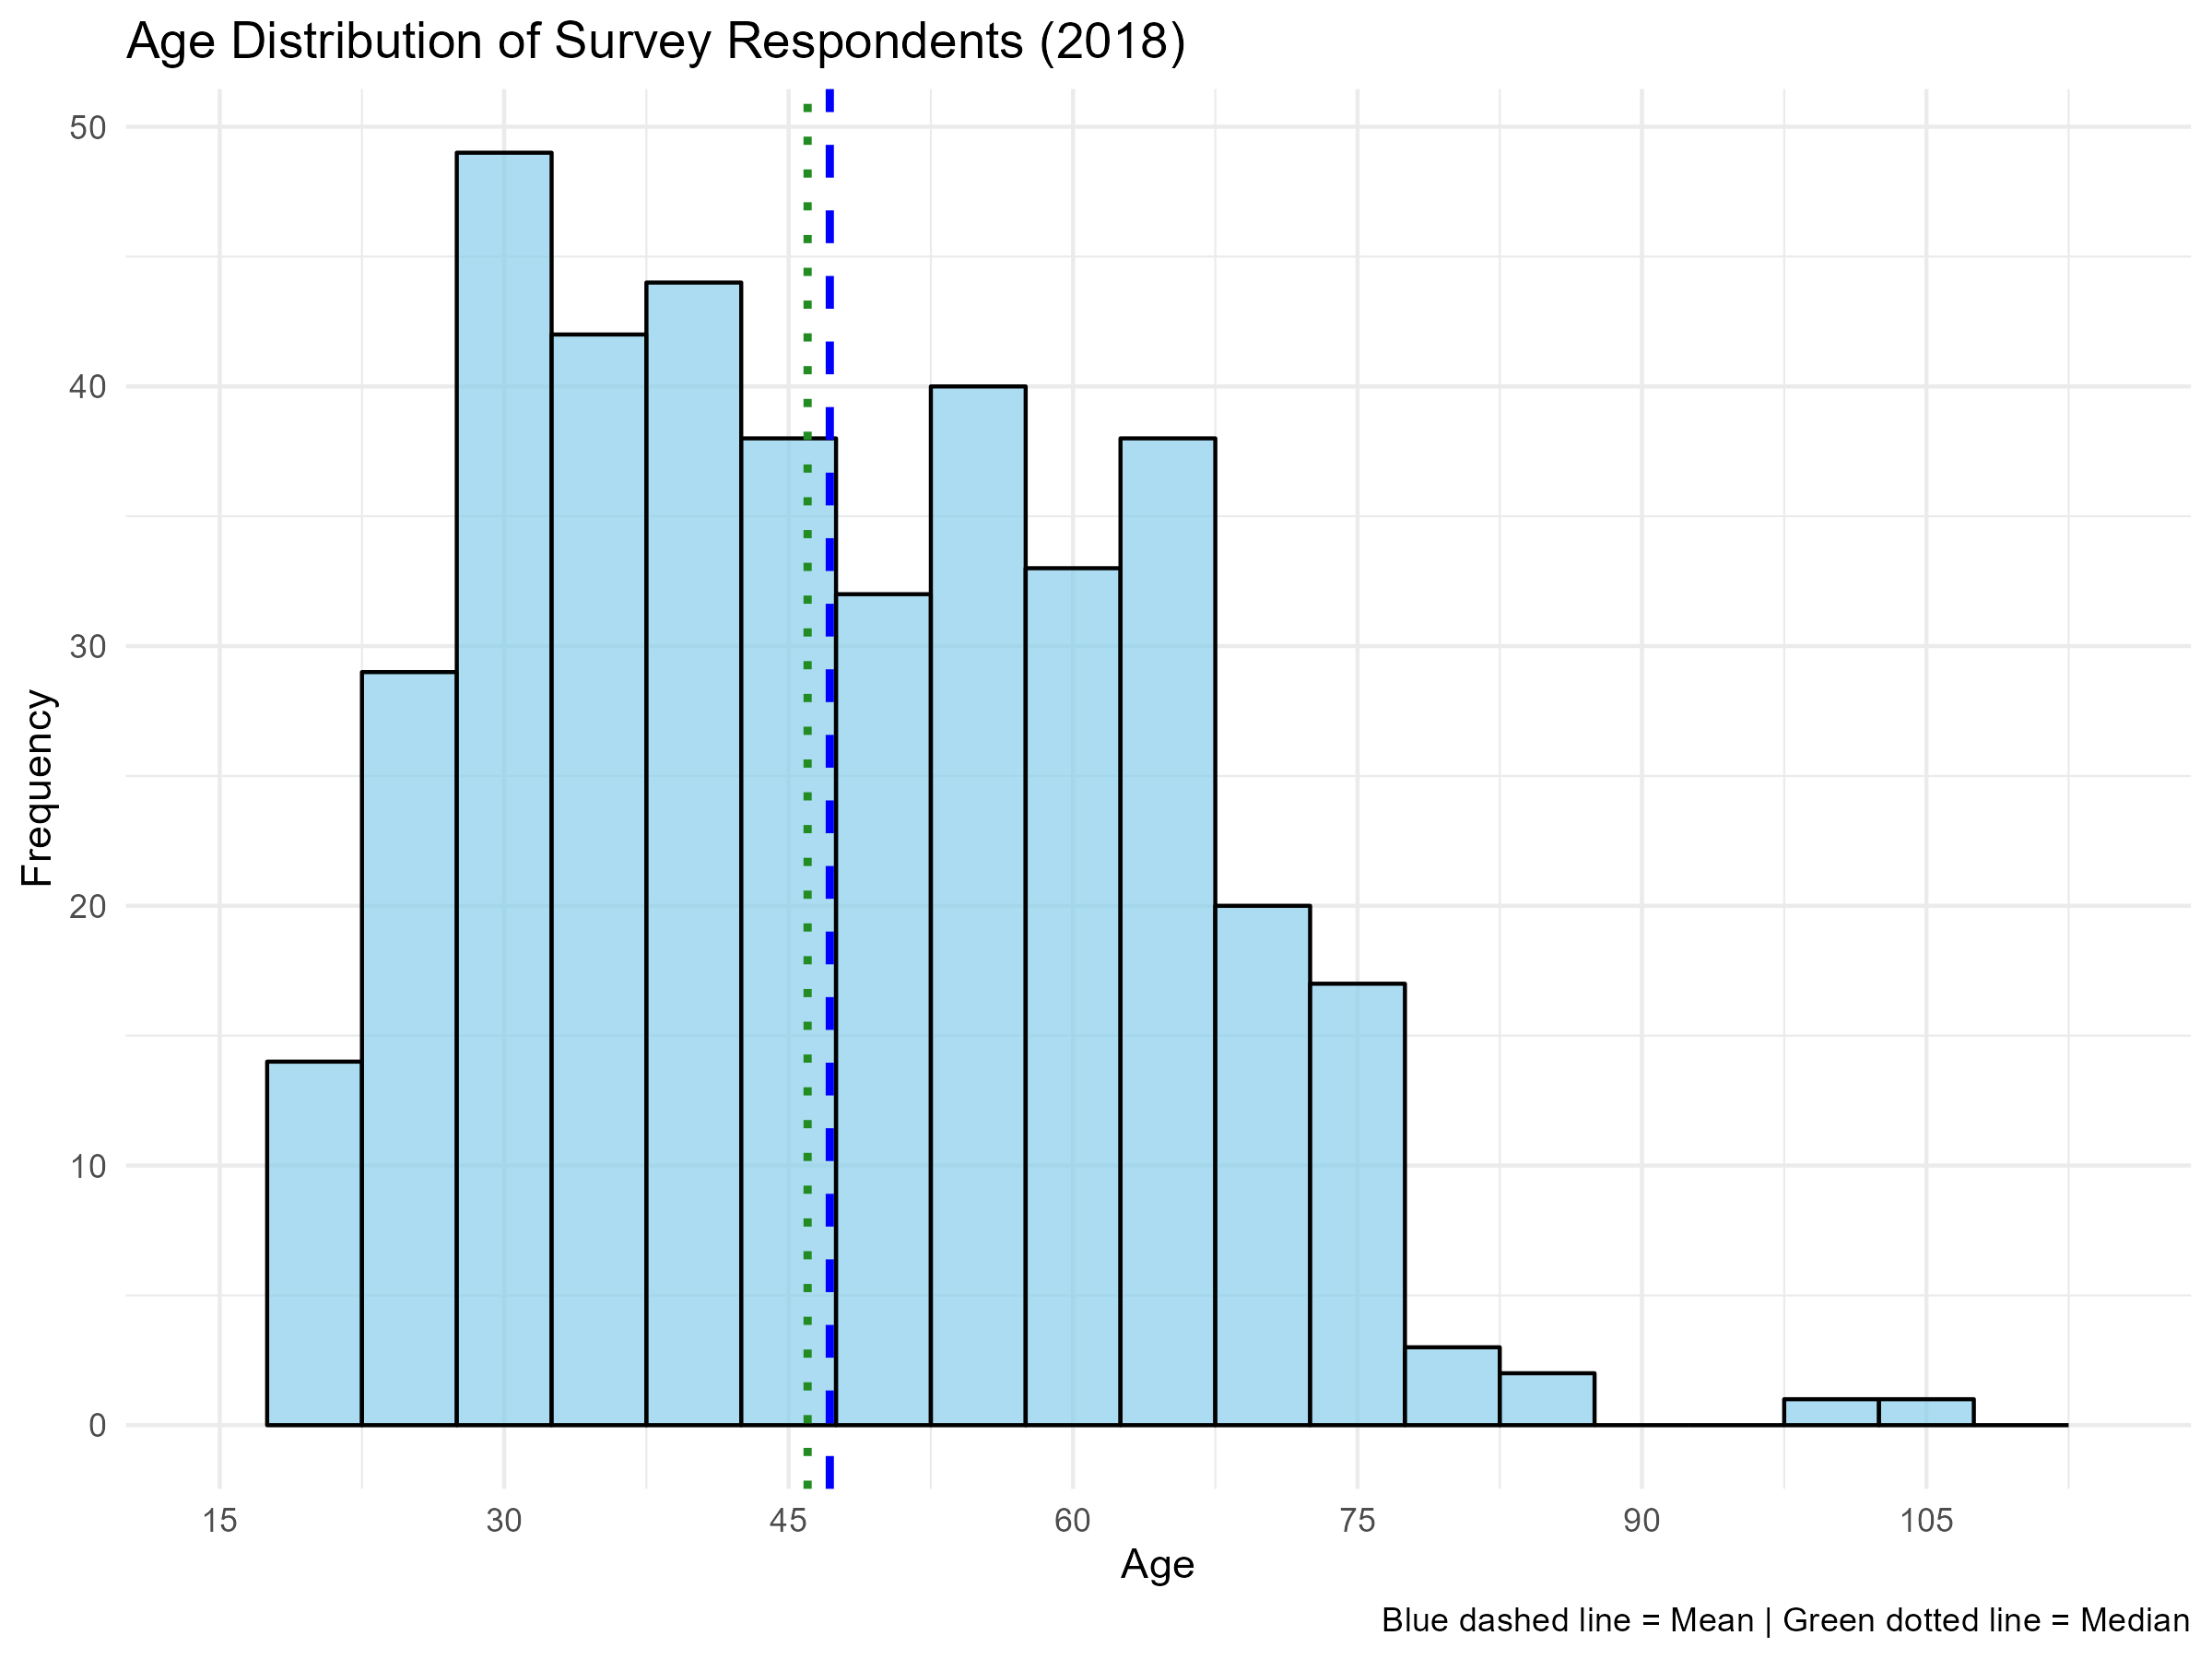
\includegraphics[width=6in,height=\textheight]{../data/03-figures_data/age_individual_plot.png}

}

\caption{\label{fig-one}The histogram shows the distribution of age
given the 2018 survey respondents.}

\end{figure}%

\paragraph{Comparison 2018 to 2021}\label{comparison-2018-to-2021}

(\textbf{table-one?}) illustrates the different age ditribution for 2018
and 2021 surveys. The major difference is that there was greater
representation of younger inviduals ranging from 18 to 23 in 2021
compared to 2018. The remaining age groups were not very different.

\begin{table}
\centering
\begin{tabular}[t]{l|r|r}
\hline
Age Group & 2018 Percentage & 2021 Percentage\\
\hline
18-23 & 4 & 11\\
\hline
24-39 & 33 & 30\\
\hline
40-55 & 30 & 26\\
\hline
56+ & 33 & 33\\
\hline
\end{tabular}
\end{table}

This table highlights the age distribution of survey respondents in 2018
and 2021.

\subsubsection{Highest Level of Education
Completed}\label{highest-level-of-education-completed}

\paragraph{Individual 2018}\label{individual-2018-1}

Figure~\ref{fig-two} illustrates the distribution of survey respondents
by their highest level of education attained. The most frequently
reported education levels are ``Completed undergraduate degree'' and
``Post graduate/professional school,'' with both categories having a
noticeably higher frequency compared to others, indicating a
well-educated respondent population. In contrast, fewer respondents
reported ``Some community college, vocational, trade school'' and
``Completed community college, vocational, trade school,'' suggesting
these levels are less common among participants. Additionally, a small
portion of respondents preferred not to disclose their education level.
This distribution highlights a skew toward higher educational attainment
within the sample, which may influence responses related to
socio-economic factors and other survey topics.

\begin{figure}

\centering{

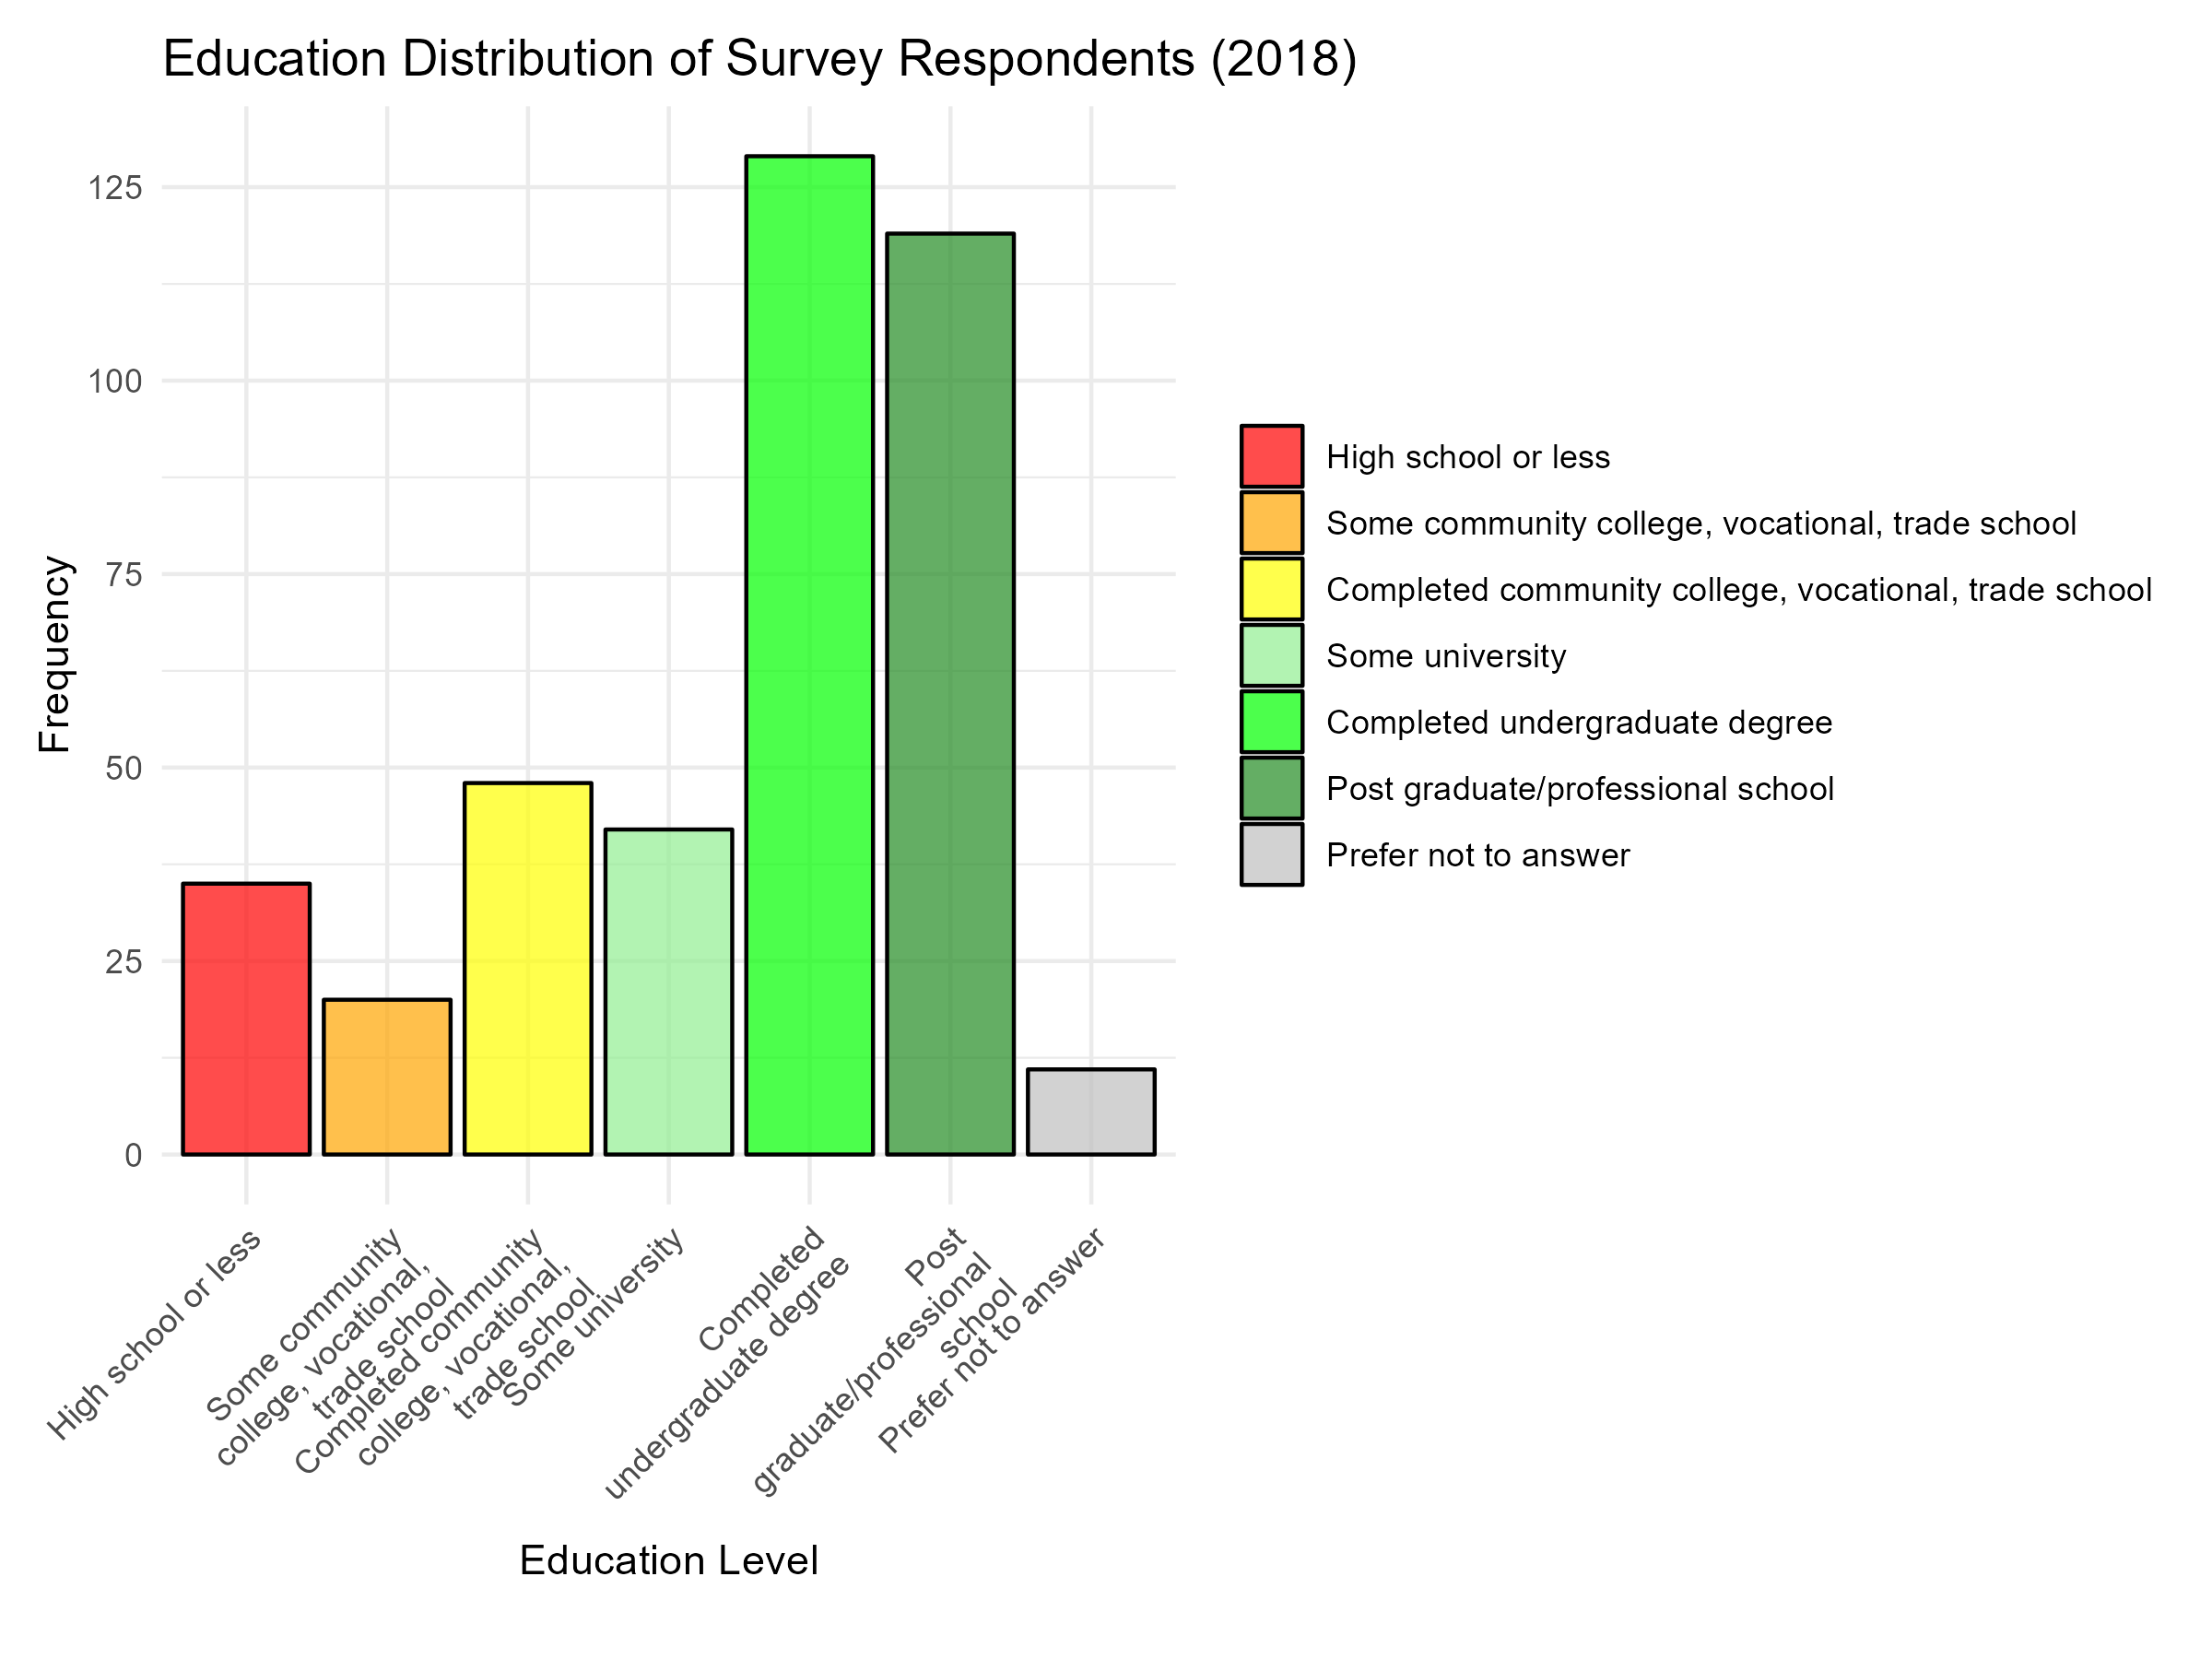
\includegraphics[width=6in,height=\textheight]{../data/03-figures_data/educ_individual_plot.png}

}

\caption{\label{fig-two}The histogram shows the distribution of
education levels of 2018 survey respondents.}

\end{figure}%

\paragraph{Comparison 2018 to 2021}\label{comparison-2018-to-2021-1}

(\textbf{table-two?}) illustrates respondant education level in 2018 and
2021 respectively. Please note, the categories of education level are
different for 2018 and 2021 as these were different surveys and
categories were updated in 2021. Despite this, we are still able to make
comparisons. Individuals with high school diplomas or less account for 9
for 2018 and 38 for 2021 (addition of less than highs school and high
school or equivalent categories). This could indicate that the younger
population was included more in the 2021 suvey or that less education
individuals were surveyed. Additionally, its not super clear howver
those with a post graduate or professional degree accounted for 29
percent in 2018 and 35 percent in 2021. This illustrates that more
educated inviduals responded to the 2021 survey.

\begin{table}
\centering
\begin{tblr}[         %% tabularray outer open
]                     %% tabularray outer close
{                     %% tabularray inner open
colspec={Q[]Q[]Q[]Q[]},
}                     %% tabularray inner close
\toprule
Education Level  & 2018 Percentage & Education Level & 2021 Percentage \\ \midrule %% TinyTableHeader
High school or less                                   &  9 & Less than high school                                                 &  6 \\
Some community college, vocational, trade school      &  5 & High School or equivalent                                             & 32 \\
Completed community college, vocational, trade school & 12 & Degree or diploma from a college or university                        & 26 \\
Some university                                       & 10 & Graduate or professional degree (examples: Master, PhD, MD or LLB/JD) & 35 \\
Completed undergraduate degree                        & 32 & Prefer not to answer                                                  &  1 \\
Post graduate/professional school                     & 29 & DK/NS                                                                 &  0 \\
Prefer not to answer                                  &  3 &                                                                       & NA \\
\bottomrule
\end{tblr}
\end{table}

This table highlights the education distribution of survey respondents
in 2018 and 2021.''

\subsubsection{Extent Feel Informed}\label{extent-feel-informed}

\paragraph{Individual 2018}\label{individual-2018-2}

Figure~\ref{fig-three} depicts the distribution of self-reported climate
change knowledge among survey respondents in 2018. The majority of
participants identified as ``Very informed,'' making this the most
prevalent category by a significant margin. A moderate number of
respondents reported being ``Not very informed,'' while a smaller yet
noticeable group described themselves as ``Extremely informed.'' In
contrast, the categories ``Not at all informed'' and ``Not very
informed'' have the lowest frequencies, with ``Not at all informed''
being particularly rare. This distribution suggests that most
respondents possess a relatively high level of awareness about climate
change, with very few indicating a lack of knowledge on the topic.

\begin{figure}

\centering{

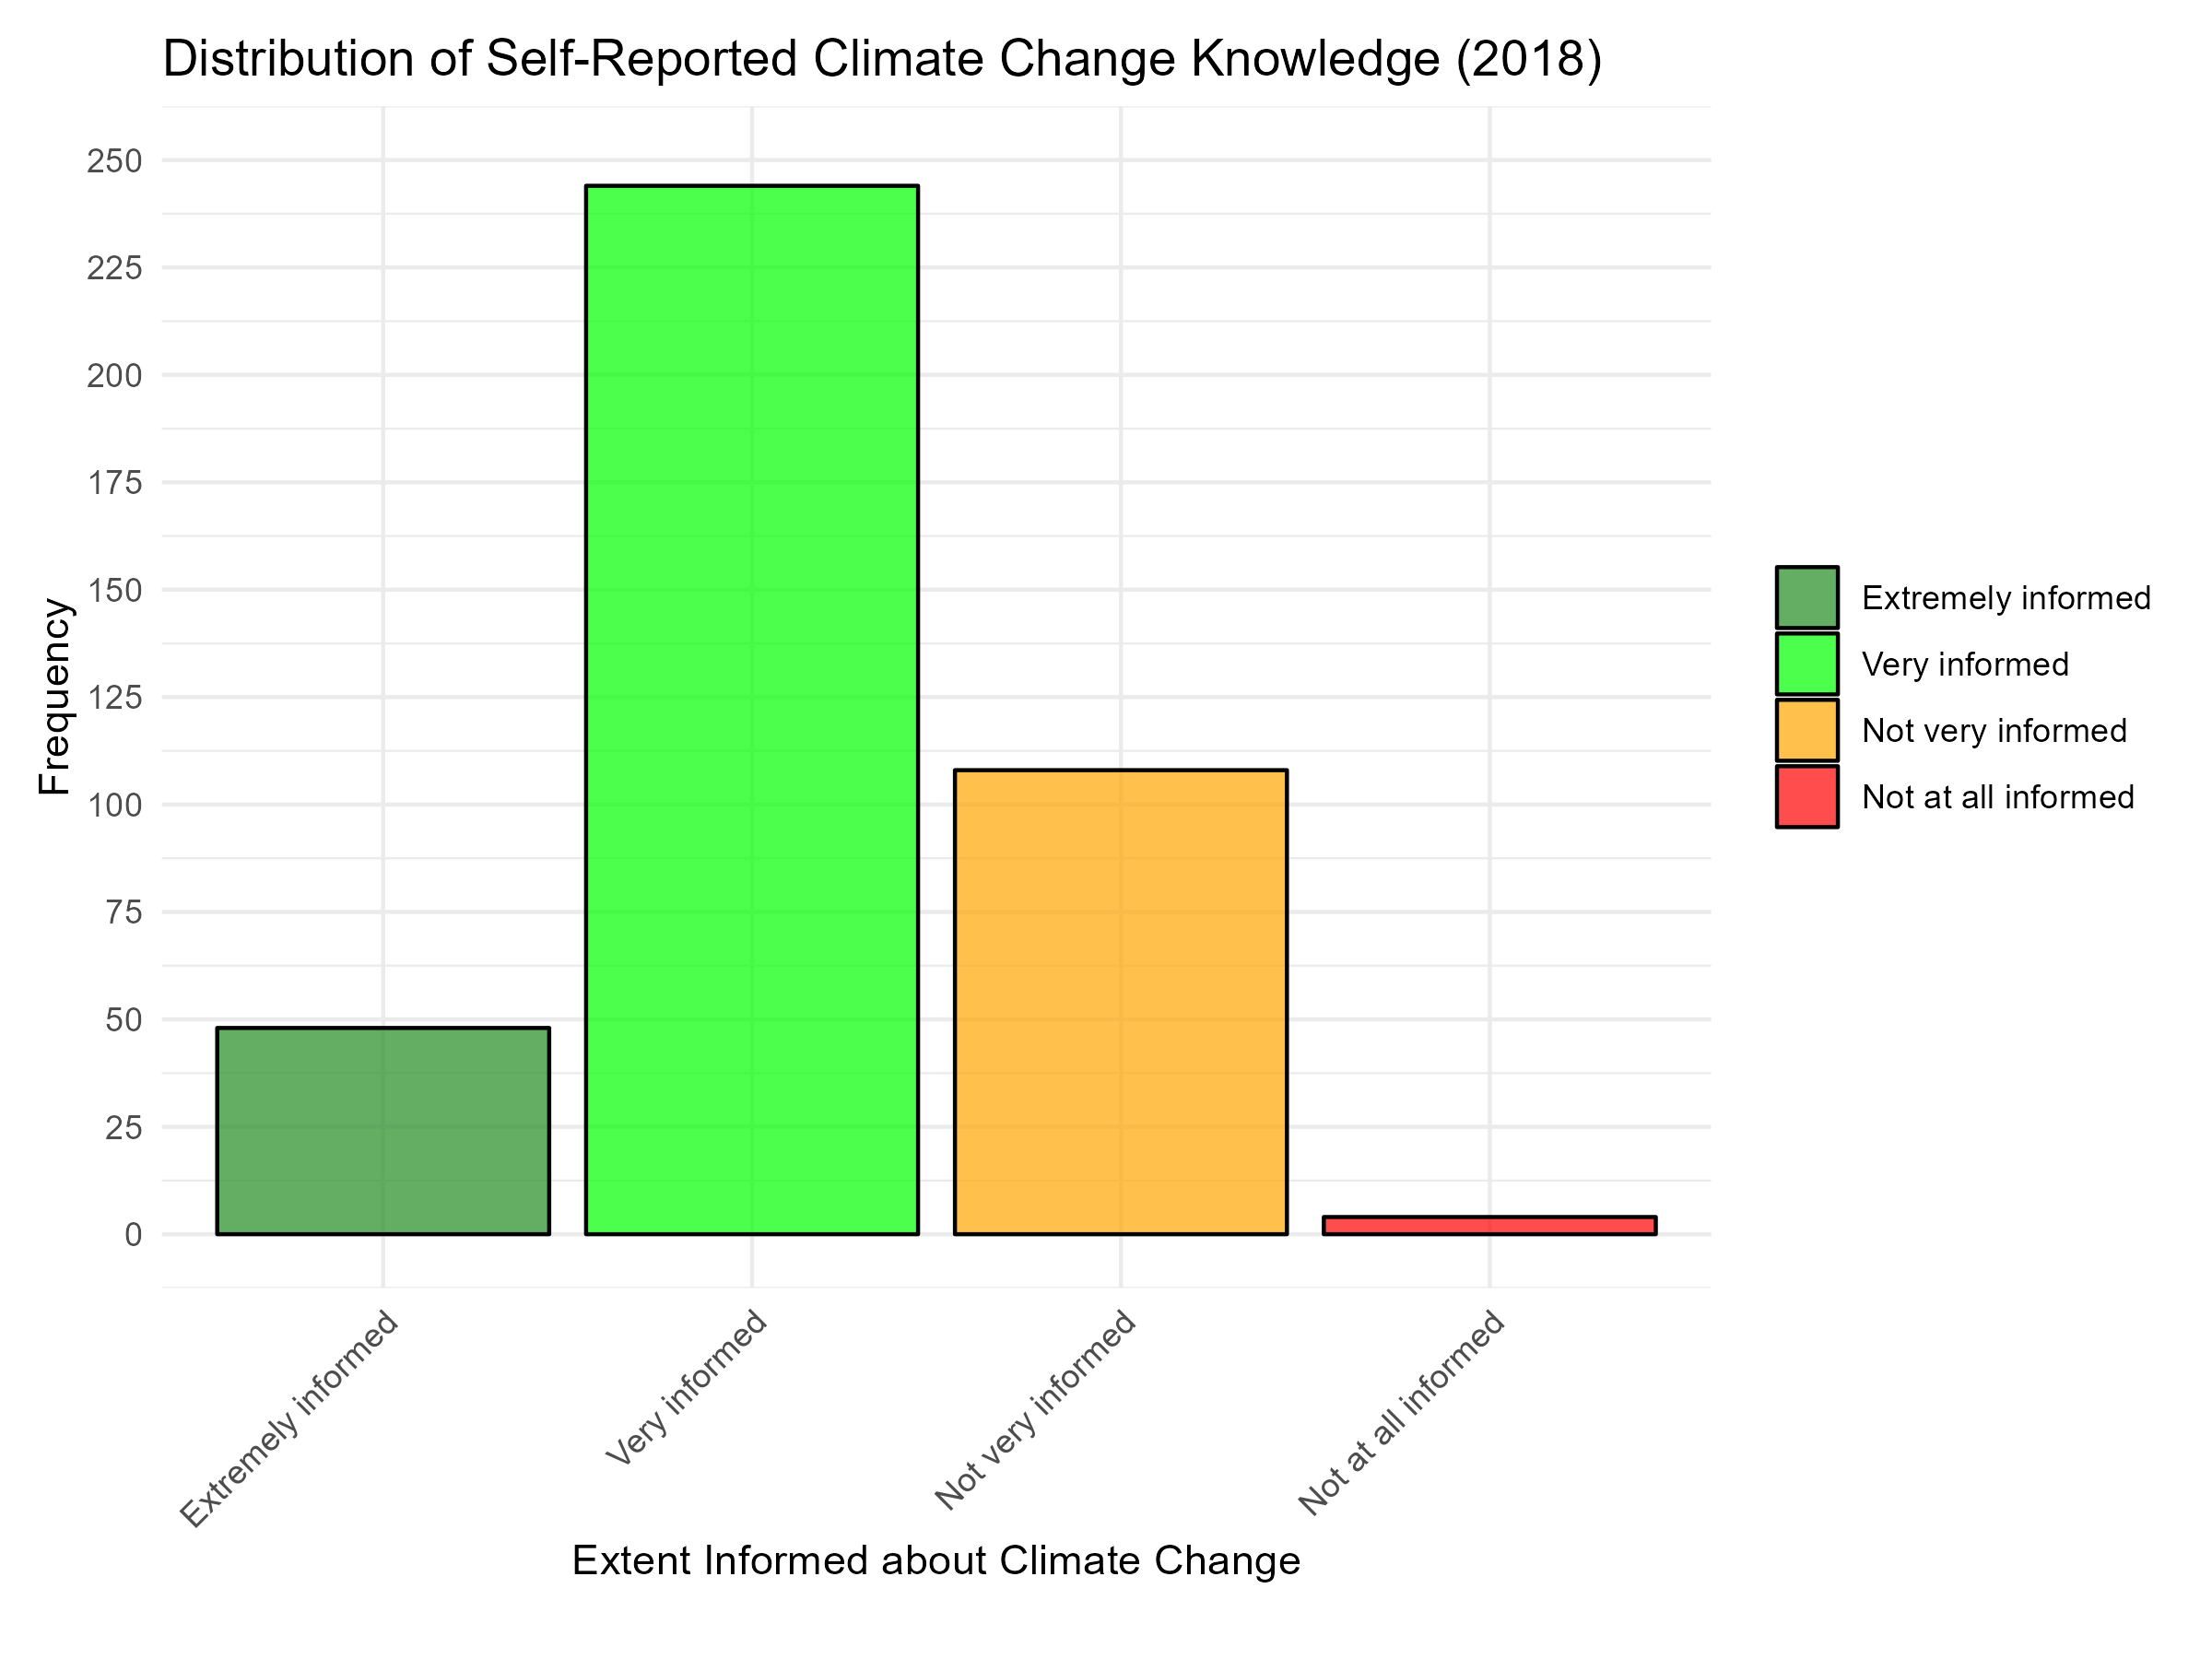
\includegraphics[width=6in,height=\textheight]{../data/03-figures_data/informed_individual_plot.png}

}

\caption{\label{fig-three}The histogram shows the distribution of
self-reported climate change knowledge among 2018 survey respondents.}

\end{figure}%

\paragraph{Comparison 2018 to 2021}\label{comparison-2018-to-2021-2}

(\textbf{table-three?}) illustrates the self-reported level of extent
inviduals feel informed about climate change and climate action for 2018
and 2021. In 2018, the large marjority of individuals say they are very
informed with 60 percent and the follwoign category is not very informed
with 27 percent. In 2021, The majority of inividuals also say they are
very informed but to a lesser degree with 48 percent and this is closely
followed by only a little informed with 37 percent. There is a trend
that invidiusls in 2018 reported greater levels of knowldege about
climate change whereas 2021 illstrates a more even split between very
informed and only little informed, portraying that fewer individuals
have adequate knowledge about climate change.

\begin{table}
\centering
\begin{tabular}[t]{l|l|l|l}
\hline
Extent Informed & 2018 Percentage & Extent Informed & 2021 Percentage\\
\hline
Extremely informed & 12 & Extremely informed & 13\\
\hline
Very informed & 60 & Very informed & 48\\
\hline
Not very informed & 27 & Only a little informed & 37\\
\hline
Not at all informed & 1 & Not at all informed & 2\\
\hline
\end{tabular}
\end{table}

This table highlights the extent feel informed distribution of survey
respondents in 2018 and 2021.

\subsubsection{Best Mode of Delivery}\label{best-mode-of-delivery}

\paragraph{Individual 2018}\label{individual-2018-3}

The analysis of the best method for delivering climate change
information portrayed in Figure~\ref{fig-four} revealed that the
majority of individuals in the 2018 dataset preferred receiving
information firstly from advertising campaigns with about 55 percent,
newsletters with about 52 percent, followed by the toronto website wiht
about 46 percent. On the other side of the spectrum, few said they were
uninterested in receiving climate action information with about 5
percent, about 12 percent indicated twitter and then 17 percent
mentioned instagram. Overall social media platforms Facebook, Instagram
and Twtitter were less popular methods of communciation. This could be
because the survey only included individals over the age of 18.
Moreover, the median sample was in the 40s.

\begin{figure}

\centering{

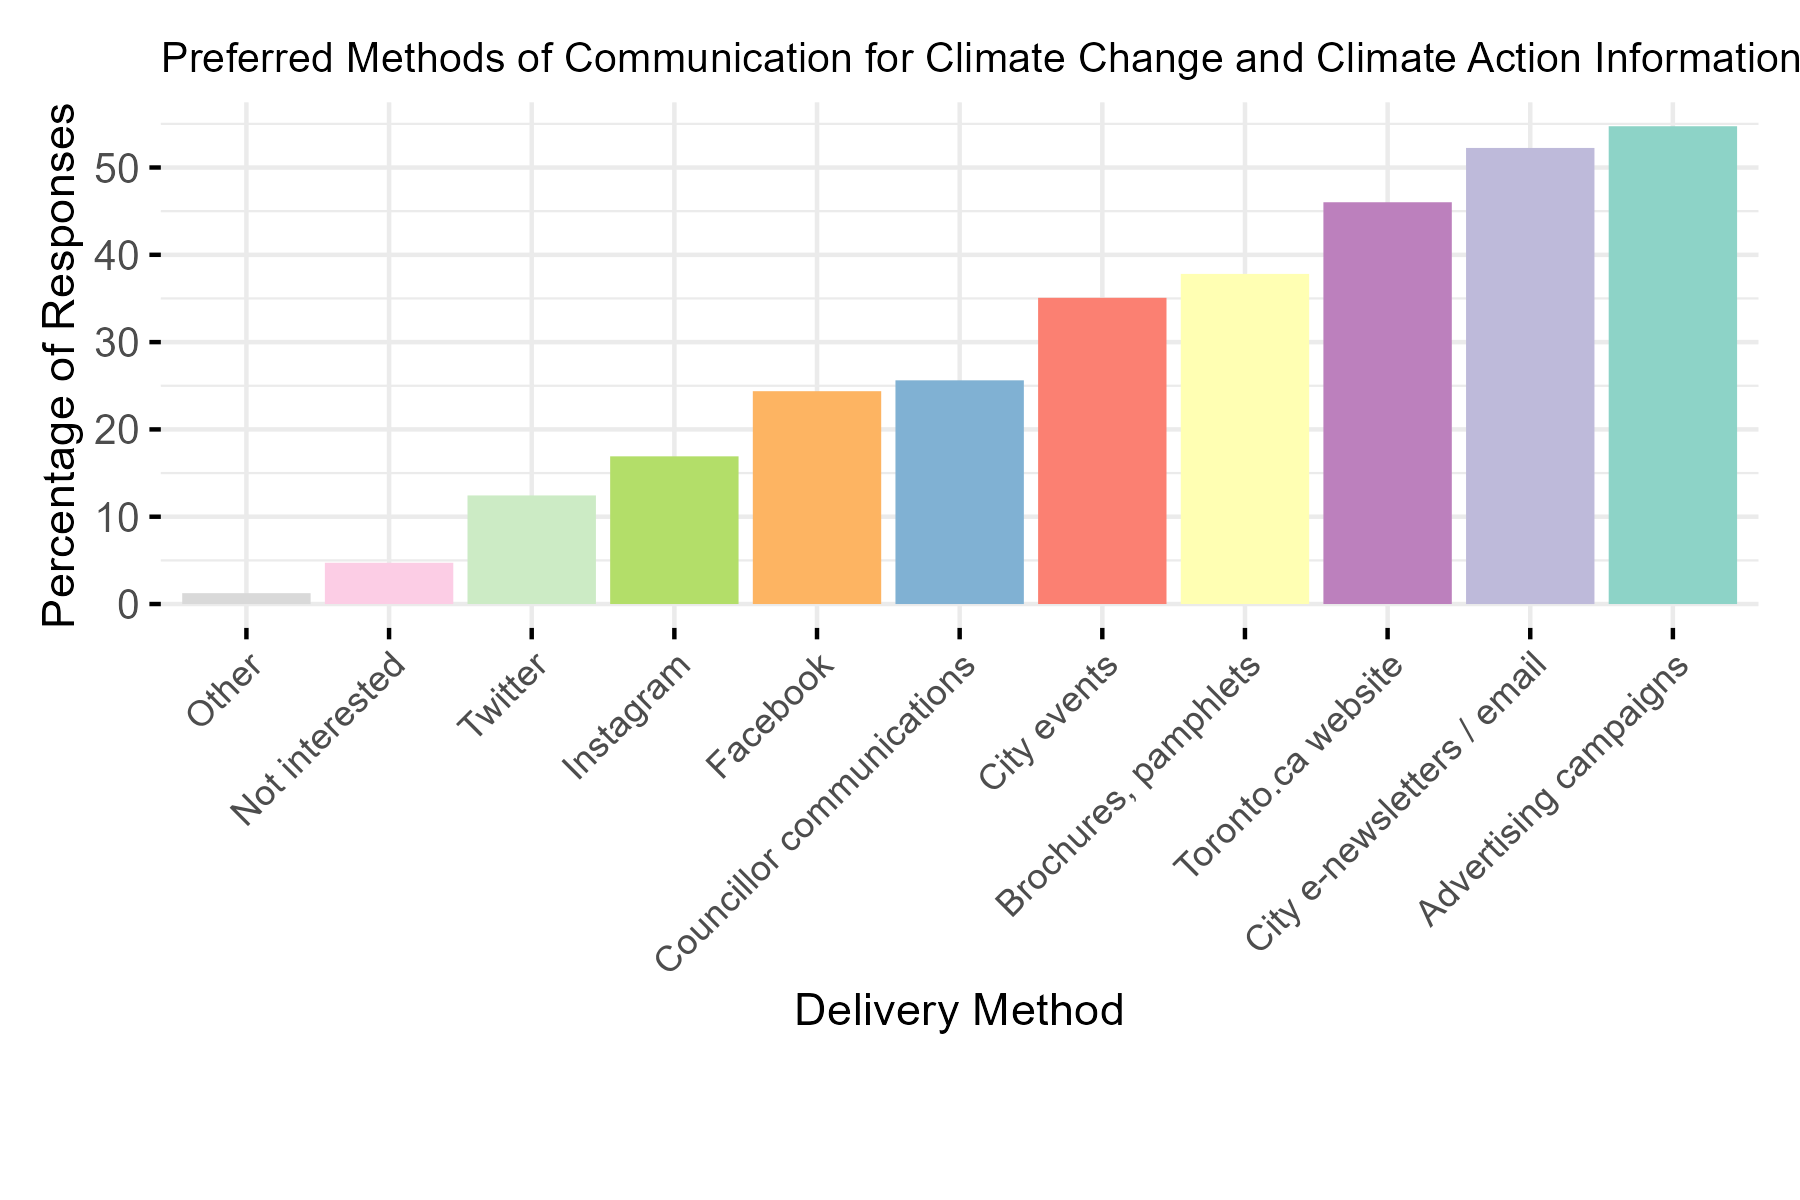
\includegraphics[width=6in,height=\textheight]{../data/03-figures_data/communication_18_plot.png}

}

\caption{\label{fig-four}The stacked bar plot illustrates the preferred
methods of communication for receiving information about climate change
and climate action.}

\end{figure}%

\paragraph{Comparison 2018 to 2021}\label{comparison-2018-to-2021-3}

(\textbf{table-four?}) compares responses from 2018 and 2021 surverys
regarding the best method of delivering information on climate change
and climate action. Aside from the additon of four options to the 2021
survey, both surveys questions are the same. The leading category for
2018 is advertising campaigns with 55 percent, closely followed by
newsletter emails with 52 percent and the Toronto website with 46. The
2021 survey illustrates a consistent trend with the same platforms as
the top method of delivering information, specifically the Toronto
website with 44 percent, then enewsletter emails with 43 percent and
advertising campains at 42 percent. These top methods of communciation
are more evenly spread out than the 2018 survey results. Social media
platforms namely twitter, facebook and instagram all increased in the
2021 survey. Notable decreases in term of percentage from 2018 to 2021
include events, enewsletter emails, advertising campaigns, brochures and
pamphlets. The new category of BetterHomesTO.ca webiste accounts for 15
percent of votes for the 2021 survey.

\begin{table}
\centering
\begin{tabular}[t]{l|l|l|l}
\hline
Communication Method & 2018 Percentage & Communication Method & 2021 Percentage\\
\hline
Toronto.ca website & 46 & Toronto.ca website & 44\\
\hline
Events & 35 & City of Toronto events & 31\\
\hline
Twitter & 13 & Twitter & 17\\
\hline
Facebook & 25 & Facebook & 26\\
\hline
Instagram & 17 & Instagram & 25\\
\hline
Enewsletter / email & 52 & City of Toronto e-newsletters / email & 43\\
\hline
Councillor communication & 25 & Councillor e-newsletters & 24\\
\hline
Advertising campaigns & 55 & Advertising campaigns & 42\\
\hline
Brochures / Pamphlets & 38 & Printed or online brochures, pamphlets & 31\\
\hline
Other & 1 & BetterHomesTO.ca website & 15\\
\hline
Not interested & 5 & Not interested in receiving information & 8\\
\hline
 &  & Mail/ letter & 1\\
\hline
 &  & Nothing & 1\\
\hline
 &  & Other & 0\\
\hline
 &  & Don't know & 0\\
\hline
\end{tabular}
\end{table}

This table highlights the prefered method of communication of survey
respondents in 2018 and 2021.

\subsubsection{Likelihood Taking Action}\label{likelihood-taking-action}

\paragraph{Individual 2018}\label{individual-2018-4}

The likelihood of taking action against climate change was explored by
assessing individuals' intentions and behaviors. Figure~\ref{fig-five}
illustrates self-reported likelihood of taking certain actions that
minimize climate change effects. On the x-axis, we have the nine
different climate actions and on the y-axis is the percentage. The
stacked bar chart allows understanding of how likely individuals are to
take part in the given actions. Sorting waste into the correct bins is
the action that most individuals are doing right now, accounting for 60
percent whith 24 percent saying they are very likely to take part in
this action. The next most prominent actions are walking or cycling
short distances, reduce hydro usage, reduce waste and home improvements.
40 percent of invidiuals report walking or cycling when traveling
shorter distances in the city with 22 percent reporting they are very
likely. However, 7 percent say they are very unlikely to change their
method of transportation. Reducing the amount of energy and water use is
already done by 36 percent and very likely for 29 percent only a mere 3
percent is very unlikely. Reducing personal waste such as contributing
to repurposing used products has similar percentages to responses for
reducing hydro but even fewer individuals that report they are very
unlikely to take action. Similarly, the likelihoods for making home
improvements for energy efficiency such as energy-efficient appliances,
programmable thermostat, LED lightbulbs, green or cool roof. In
contrast, the action where the least number of individuals are
contributing to is the investment of an electric or hybrid vehicle over
gas-powered vehicles with only 8 percent who currently have an energy
efficient vehicle. While 19 percetn are very likely to make this switch,
14 percent say they are very unlikely. This illustrates that buying an
electric or hybrid vehicle is action the least number of individuals are
willing to invest in despite gas-powered vehicles being a major
contributor to greenhouse gases. This action has a huge impact on the
environment and yet 41 percent of this sample say they are unlikely to
change! The second action that individuals are most unlikely to engage
in is eat less meat by incorporating more plant-based foods in their
diet with 12 percent very unlikely and 23 percent somewhat unlikely.
Only 23 percent are already consuming meat alternatives. Vegans
greenhosue gas emissions are on average 37\% lower than those who eat
meat frequently.

\begin{figure}

\centering{

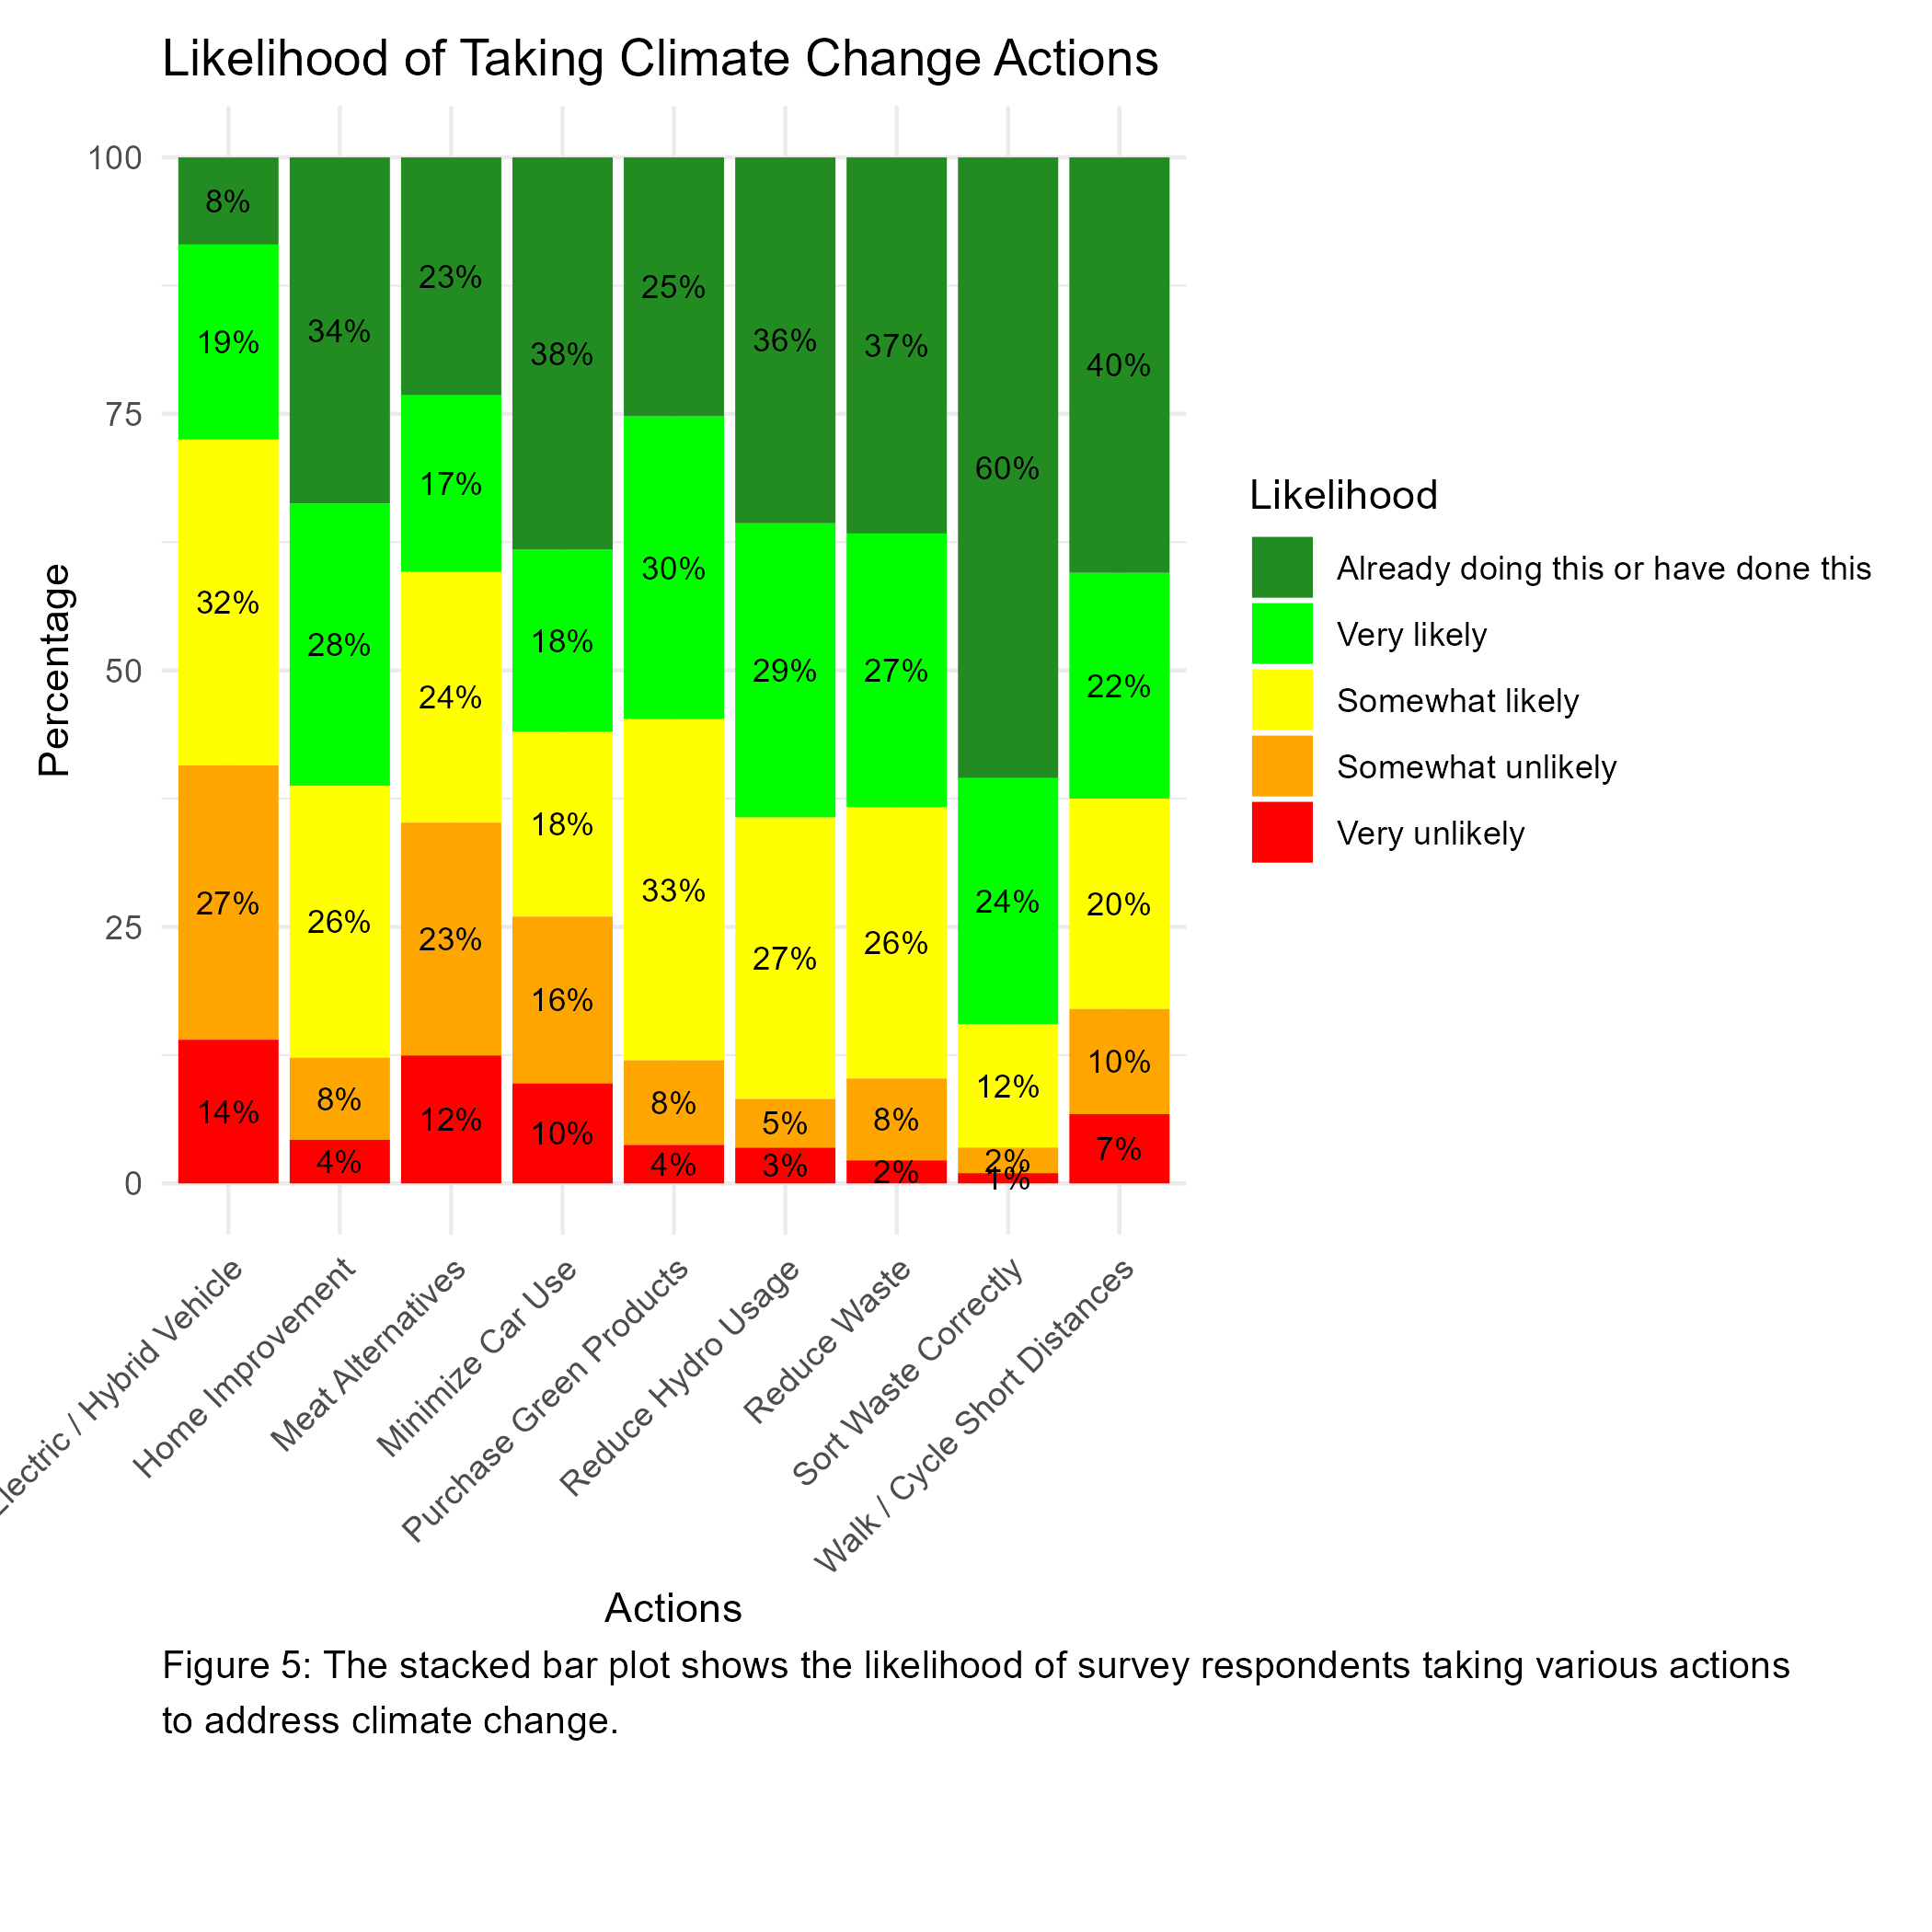
\includegraphics[width=6in,height=\textheight]{../data/03-figures_data/likelihood_individual_plot.png}

}

\caption{\label{fig-five}The stacked bar plot shows the likelihood of
survey respondents taking various actions to address climate change.}

\end{figure}%

\section{Model}\label{sec-model}

The goal of our modelling strategy is twofold. Firstly, we aim to
predict the likelihood of individuals engaging in climate-friendly
actions based on demographic variables, specifically age and education.
The actions considered include investing in electric or hybrid vehicles,
making home improvements (such as using LED lightbulbs), adopting meat
alternatives, minimizing car use, purchasing green products, reducing
hydro usage, reducing waste, sorting waste correctly, and walking or
cycling shorter distances. Secondly, we aim to understand how these
demographic characteristics influence individuals' likelihood of
adopting these behaviors.Here we describe the probability tree model
used to investigate the relationship between likelihood and the
demographic factors of age and education.

\subsection{Model set-up}\label{model-set-up}

In this analysis, we focus on predicting the likelihood of taking
climate-friendly actions based on the demographic variables of age and
education. The likelihood is measured on a five-point Likert scale,
ranging from ``Very unlikely'' to ``Already doing this or have done
this.''

\subsubsection{Model Specifications}\label{model-specifications}

We use a probability tree model to predict the likelihood of individuals
engaging in climate-friendly actions based on two key demographic
variables: age and education.

The general form of the model is:

\textbackslash begin\{align\} y\_i = \beta\_0 + \beta\_1 * Age\_i +
\beta\_2 * Education\_i + \epsilon\_i \textbackslash end\{align*\}
where:

\begin{itemize}
\tightlist
\item
  \(y_i\) represents the likelihood of individual \(i\) engaging in a
  climate-friendly actin, measured on a five point Likert scale:
\end{itemize}

\begin{enumerate}
\def\labelenumi{\arabic{enumi}.}
\tightlist
\item
  ``Very unlikely''
\item
  ``Somewhat unlikely''
\item
  ``Somewhat likely''
\item
  ``Very likely''
\item
  ``Already doing this or have done this''
\end{enumerate}

\begin{itemize}
\tightlist
\item
  \(\beta_0\) is the intercept, representing the baseline likelihood of
  taking action when all predictors are zero.
\item
  \(\beta_1\) is the coefficient for Age, representing how a one-year
  increase affects the likelihood of taking action.
\item
  \(\beta_2\) is the coefficient for Education, a categorical variable
  that is dummy-coded.
\item
  \(\epsilon_i\) is the error term, accounting for unexplained
  variation.
\end{itemize}

This model focuses on the direct effect of age and education on the
likelihood of taking climate-friendly actions, assuming a linear
relationship between these demographic variables and the outcome
variable (the likelihood of action).

\subsubsection{Model Justification}\label{model-justification}

This model was developed to explore how demographic factors such as age
and education influence individuals' likelihood of engaging in
climate-friendly behaviors. By focusing on specific climate actions like
reducing energy consumption, adopting sustainable practices, and
investing in green technologies, the model aims to provide actionable
insights for climate change interventions.

\paragraph{Response Variable}\label{response-variable}

The response variable in this analysis is the likelihood of taking
climate-friendly actions, measured using a Likert scale (1 = ``Very
unlikely'' to 5 = ``Already doing this or have done this''). This scale
captures the respondent's perceived likelihood of engaging in various
climate-friendly behaviors

\paragraph{Input Variabless}\label{input-variabless}

The input variables (predictors) include:

\begin{itemize}
\tightlist
\item
  \textbf{Age}: Previous research indicates that younger individuals may
  be more inclined to adopt climate-friendly behaviors due to increased
  environmental awareness (Leiserowitz et al., 2010; Gifford, 2013).
\item
  \textbf{Education}: Higher levels of education are often linked to
  greater awareness of environmental issues and a higher likelihood of
  adopting sustainable behaviors (Kollmuss \& Agyeman, 2002). Education
  is treated as a categorical variable and dummy-coded for analysis.
\end{itemize}

\paragraph{Model Structure}\label{model-structure}

This model assumes a linear relationship between the predictors (age and
education) and the likelihood of taking action. Specifically, the
likelihood of taking climate-friendly actions is modeled as a function
of age and education, with coefficients representing the change in the
likelihood of action associated with a unit change in each predictor.

There are no interaction terms in this model, meaning we assume that the
effects of age and education on the likelihood of taking action are
independent of each other. This simplicity ensures clear interpretation
of each predictor's individual effect on the likelihood of taking
climate-friendly actions.

\subsection{Nine Models}\label{nine-models}

We fit nine separate probability tree models, one for each
climate-friendly action we are predicting. Each model uses age and
education as the predictors to estimate the likelihood of the
corresponding action. These actions are:

\begin{enumerate}
\def\labelenumi{\arabic{enumi}.}
\tightlist
\item
  Likelihood of investing in an electric or hybrid vehicle
\item
  Likelihood of making home improvements (e.g., using LED lightbulbs)
\item
  Likelihood of adopting meat alternatives
\item
  Likelihood of minimizing car use
\item
  Likelihood of purchasing green products 6 Likelihood of reducing hydro
  usage
\item
  Likelihood of reducing waste by repurposing used products
\item
  Likelihood of sorting waste correctly
\item
  Likelihood of walking or cycling shorter distances
\end{enumerate}

Each model is built using the same structure but predicts a different
outcome variable. This approach allows us to analyze the specific impact
of age and education on each climate-friendly action.

\subsubsection{Likelihood of investing in an electric or hybrid
vehicle}\label{likelihood-of-investing-in-an-electric-or-hybrid-vehicle}

\begin{figure}[H]

{\centering 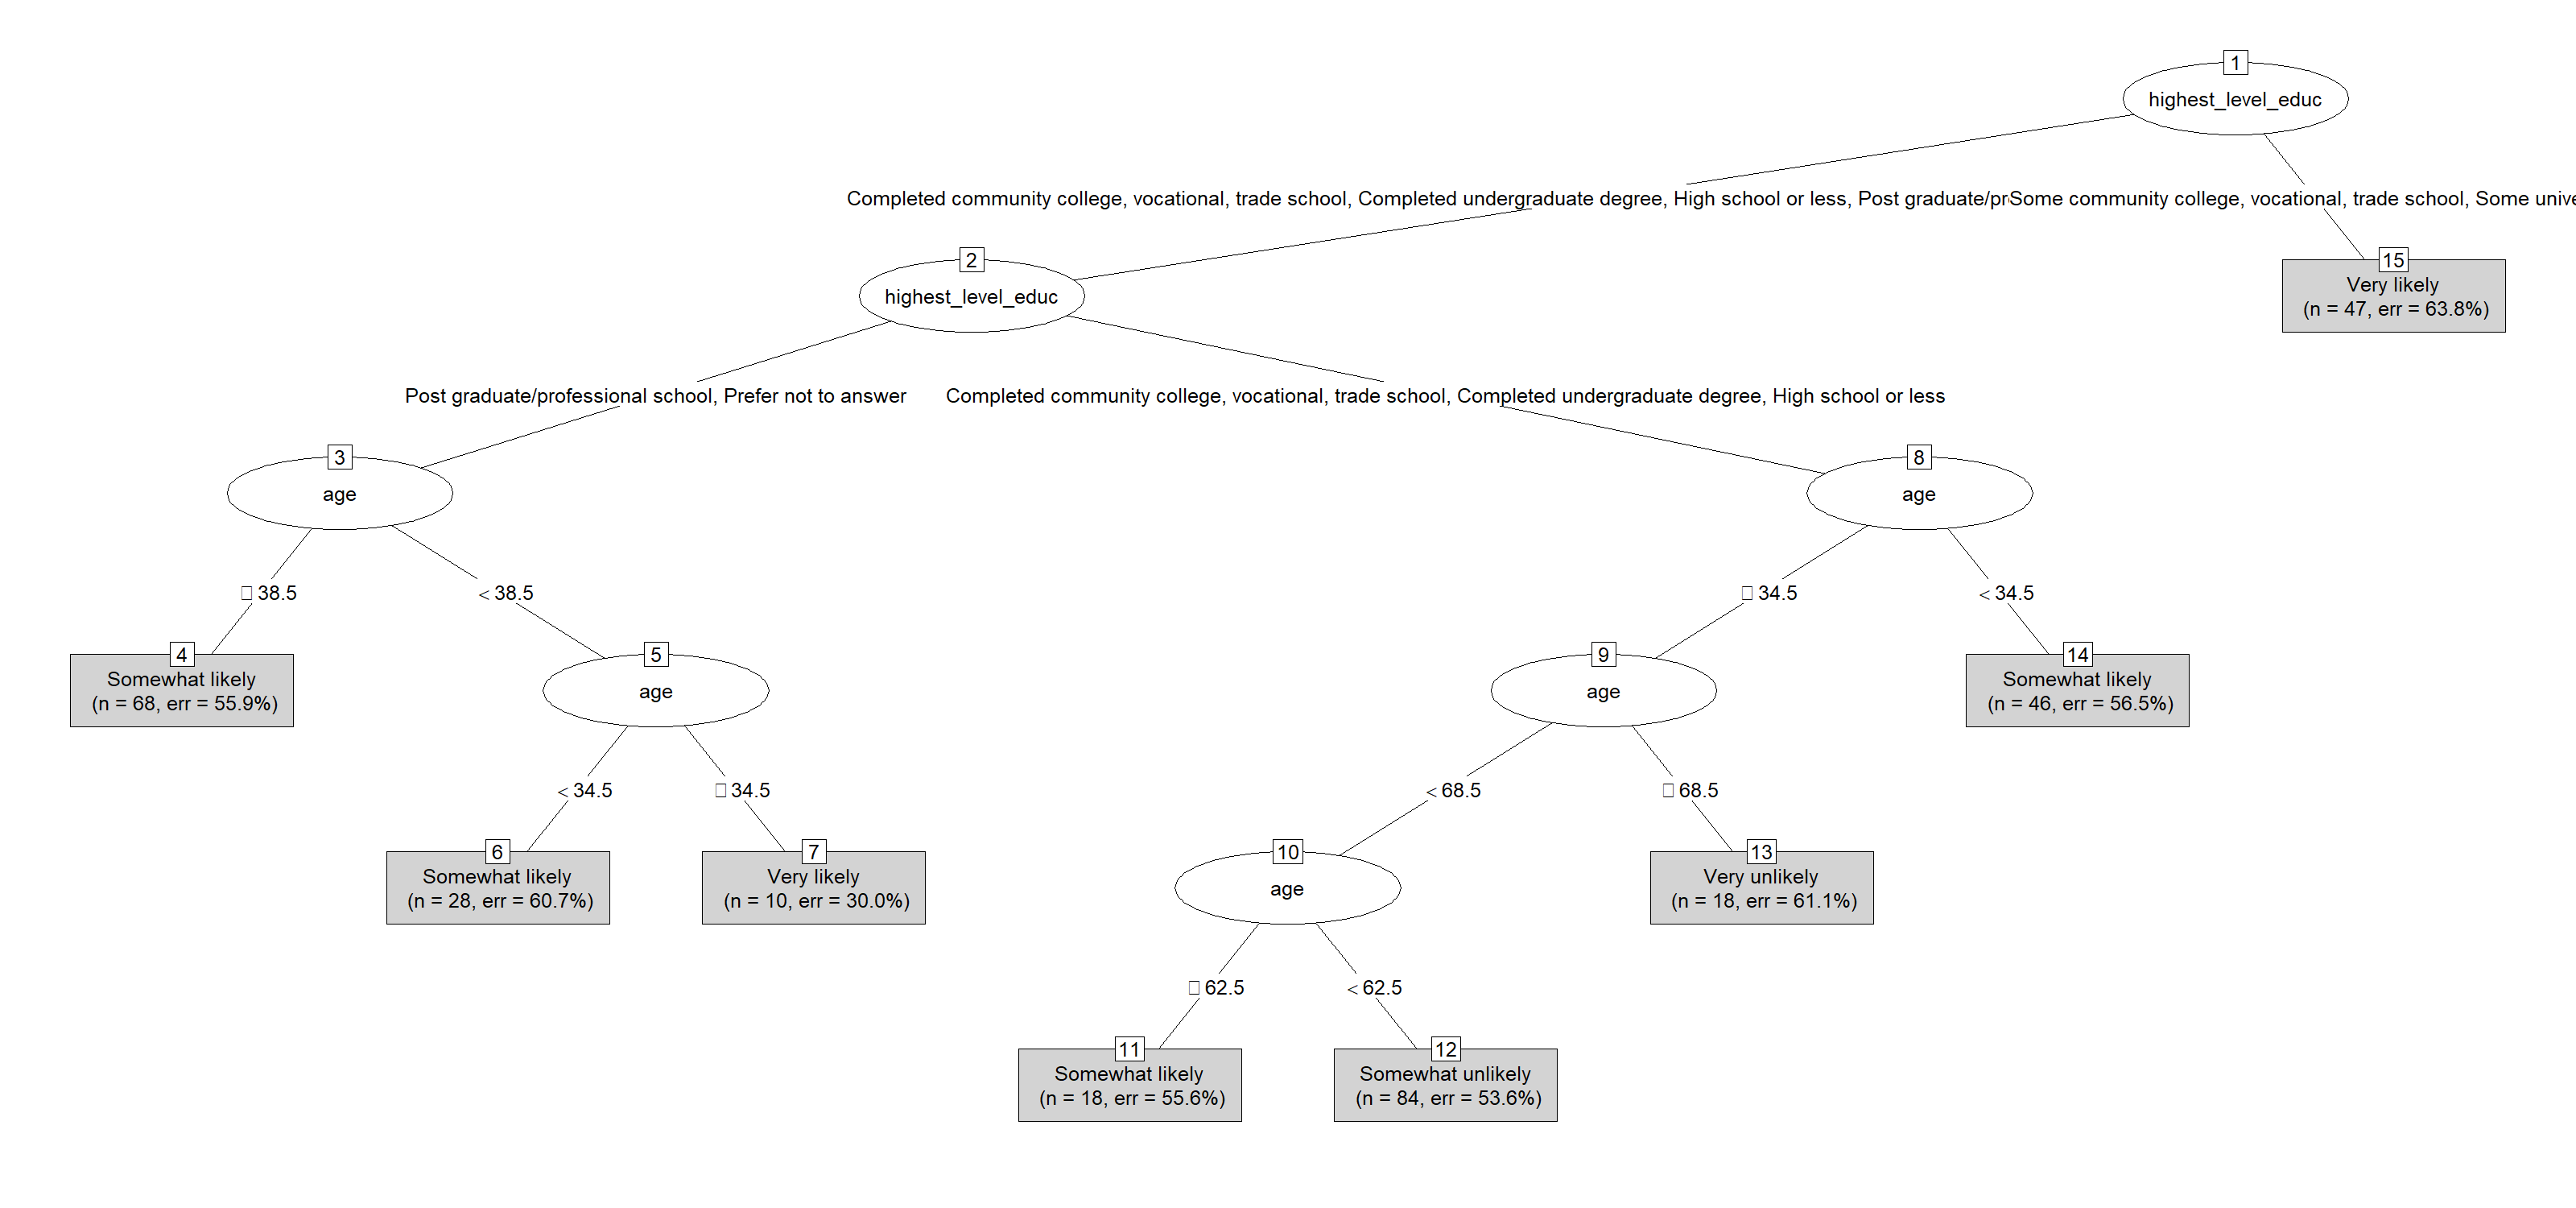
\includegraphics[width=10.67in,height=\textheight]{../data/04-model_data/vehicle_electric_tree.png}

}

\caption{Probability tree for likelihood of investing in an electric or
hybrid vehicle, predicted by age and education.}

\end{figure}%

\subsubsection{Likelihood of making home
improvements}\label{likelihood-of-making-home-improvements}

\begin{figure}[H]

{\centering 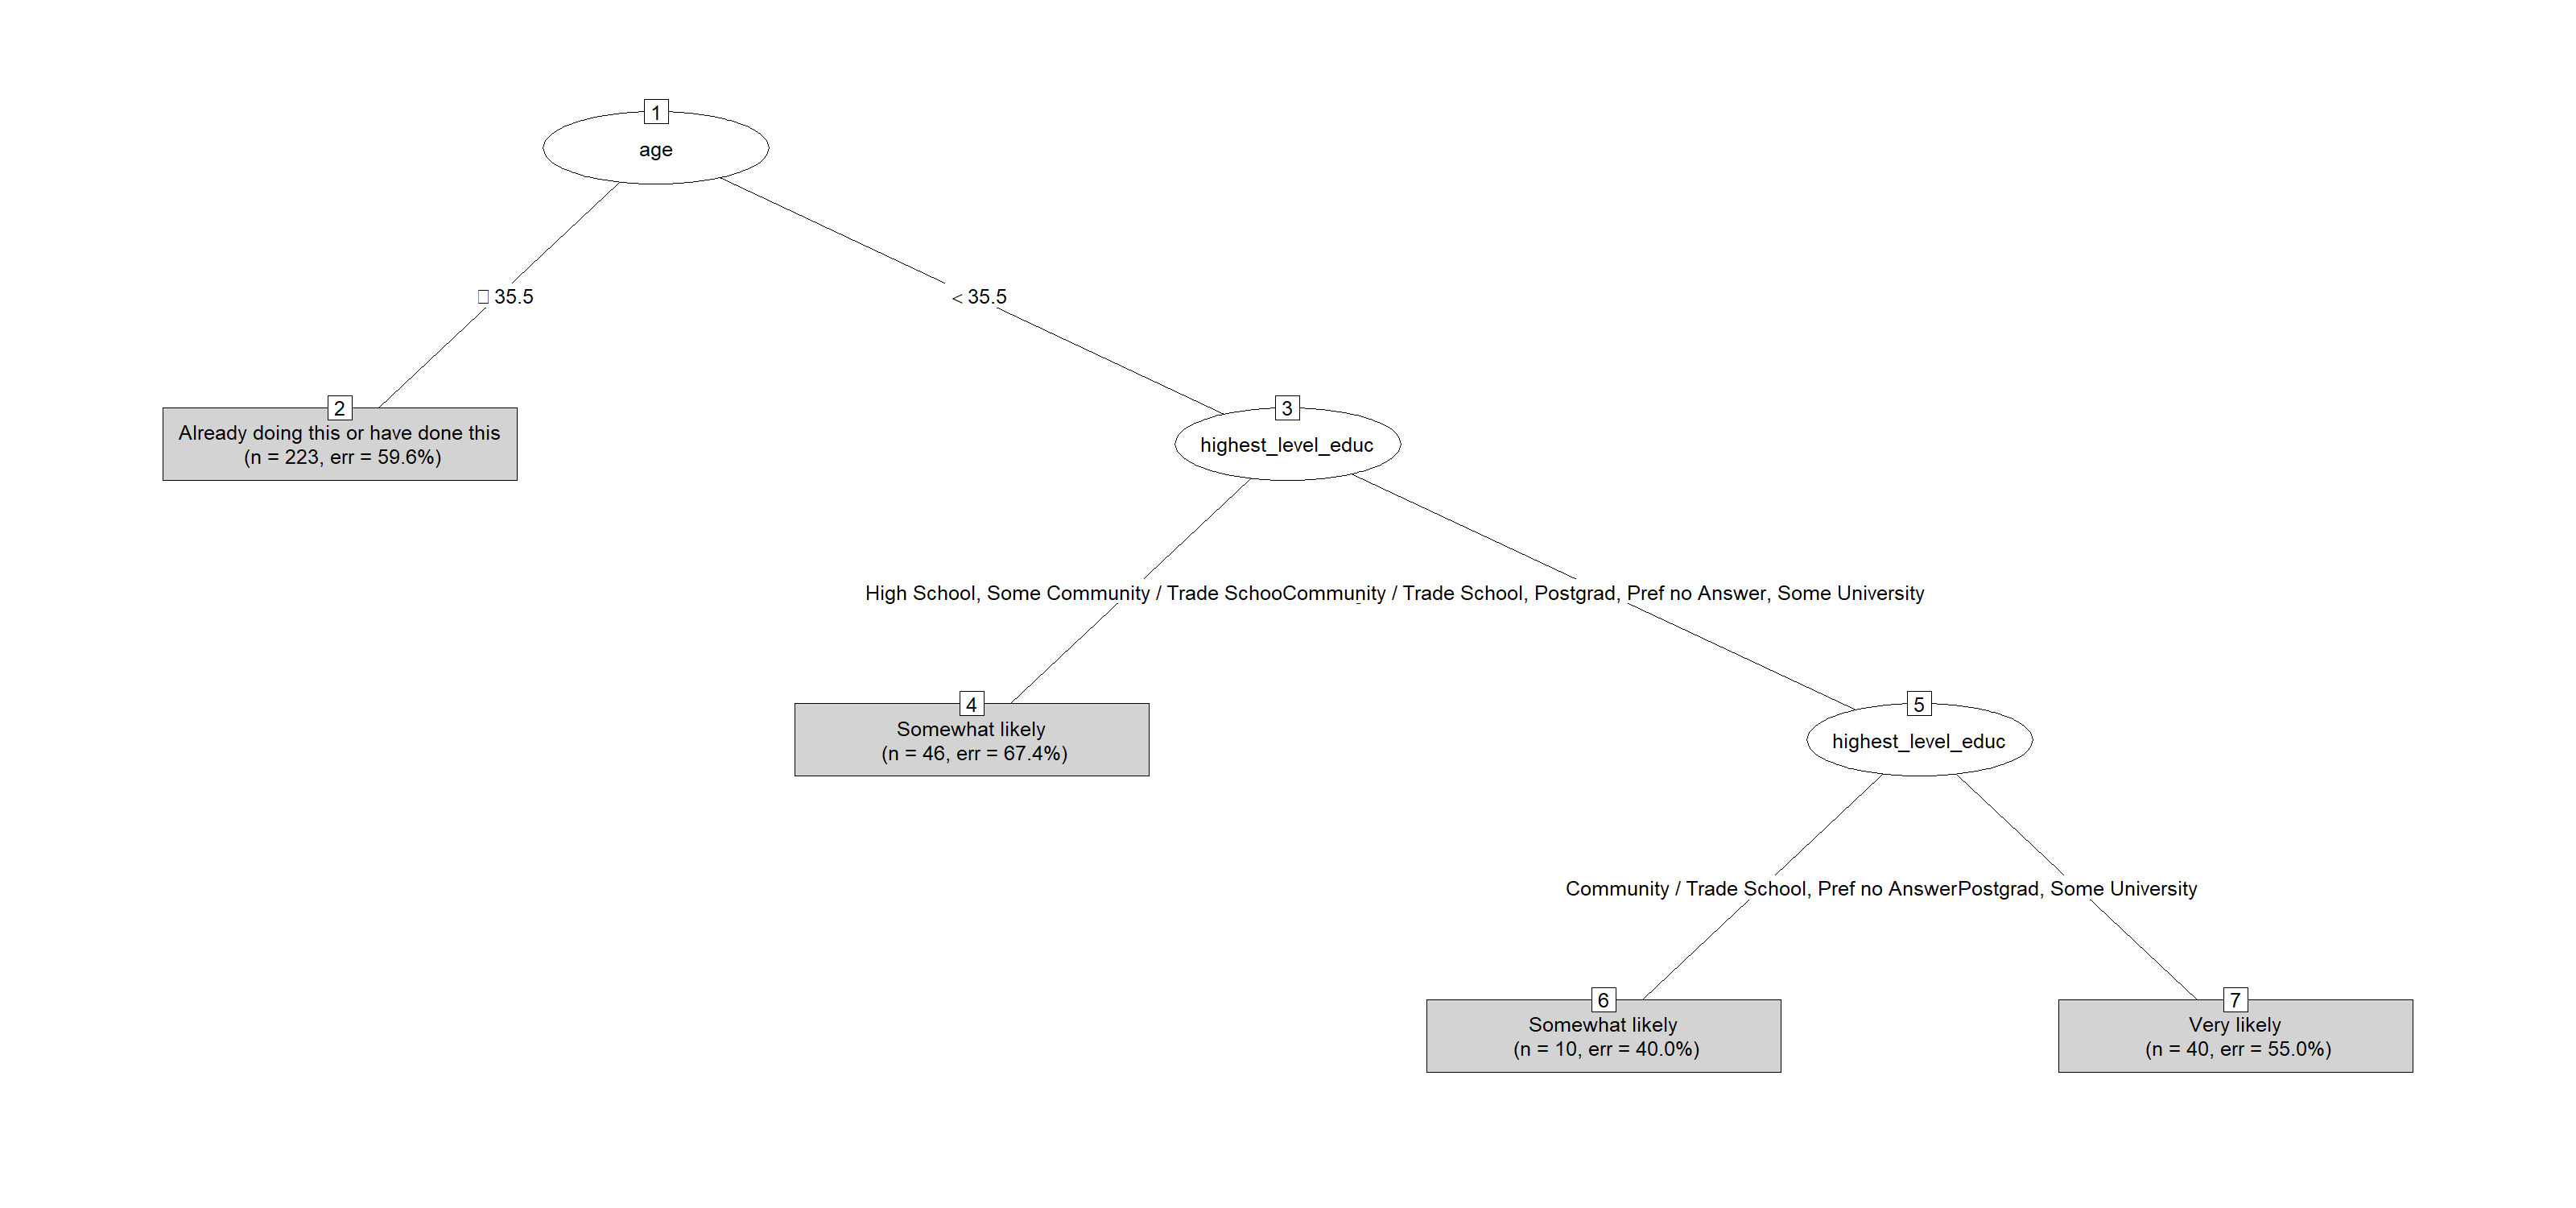
\includegraphics[width=10.67in,height=\textheight]{../data/04-model_data/home_improvement_tree.png}

}

\caption{Probability tree for likelihood of making home improvements
predicted by age and education.}

\end{figure}%

\subsubsection{Likelihood of adopting meat
alternatives}\label{likelihood-of-adopting-meat-alternatives}

\begin{figure}[H]

{\centering 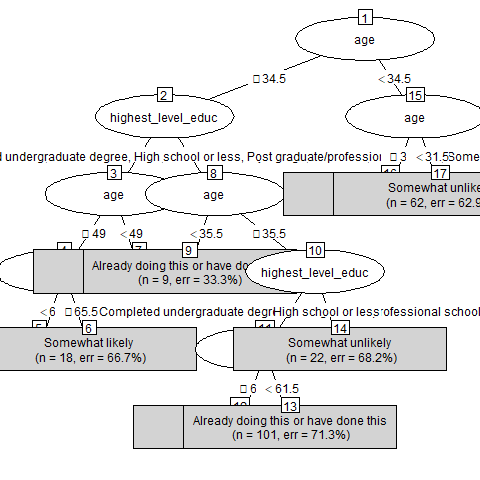
\includegraphics[width=10.67in,height=\textheight]{../data/04-model_data/protein_alternative_tree.png}

}

\caption{Probability tree for likelihood of adopting meat alternatives,
predicted by age and education.}

\end{figure}%

\subsubsection{Likelihood of minimizing car
use}\label{likelihood-of-minimizing-car-use}

\begin{figure}[H]

{\centering 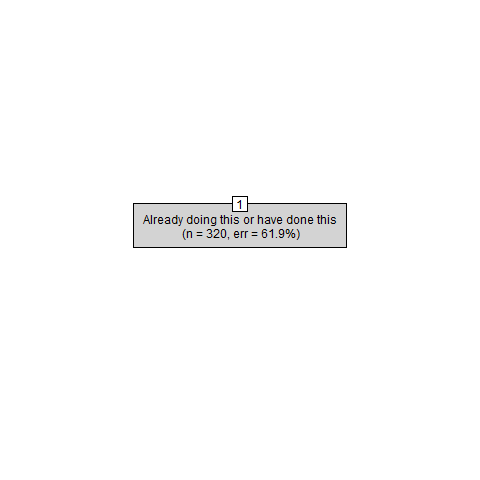
\includegraphics[width=10.67in,height=\textheight]{../data/04-model_data/minimize_car_tree.png}

}

\caption{Probability tree for likelihood of minimizing car use,
predicted by age and education.}

\end{figure}%

\subsubsection{Likelihood of purchasing green
products}\label{likelihood-of-purchasing-green-products}

\begin{figure}[H]

{\centering 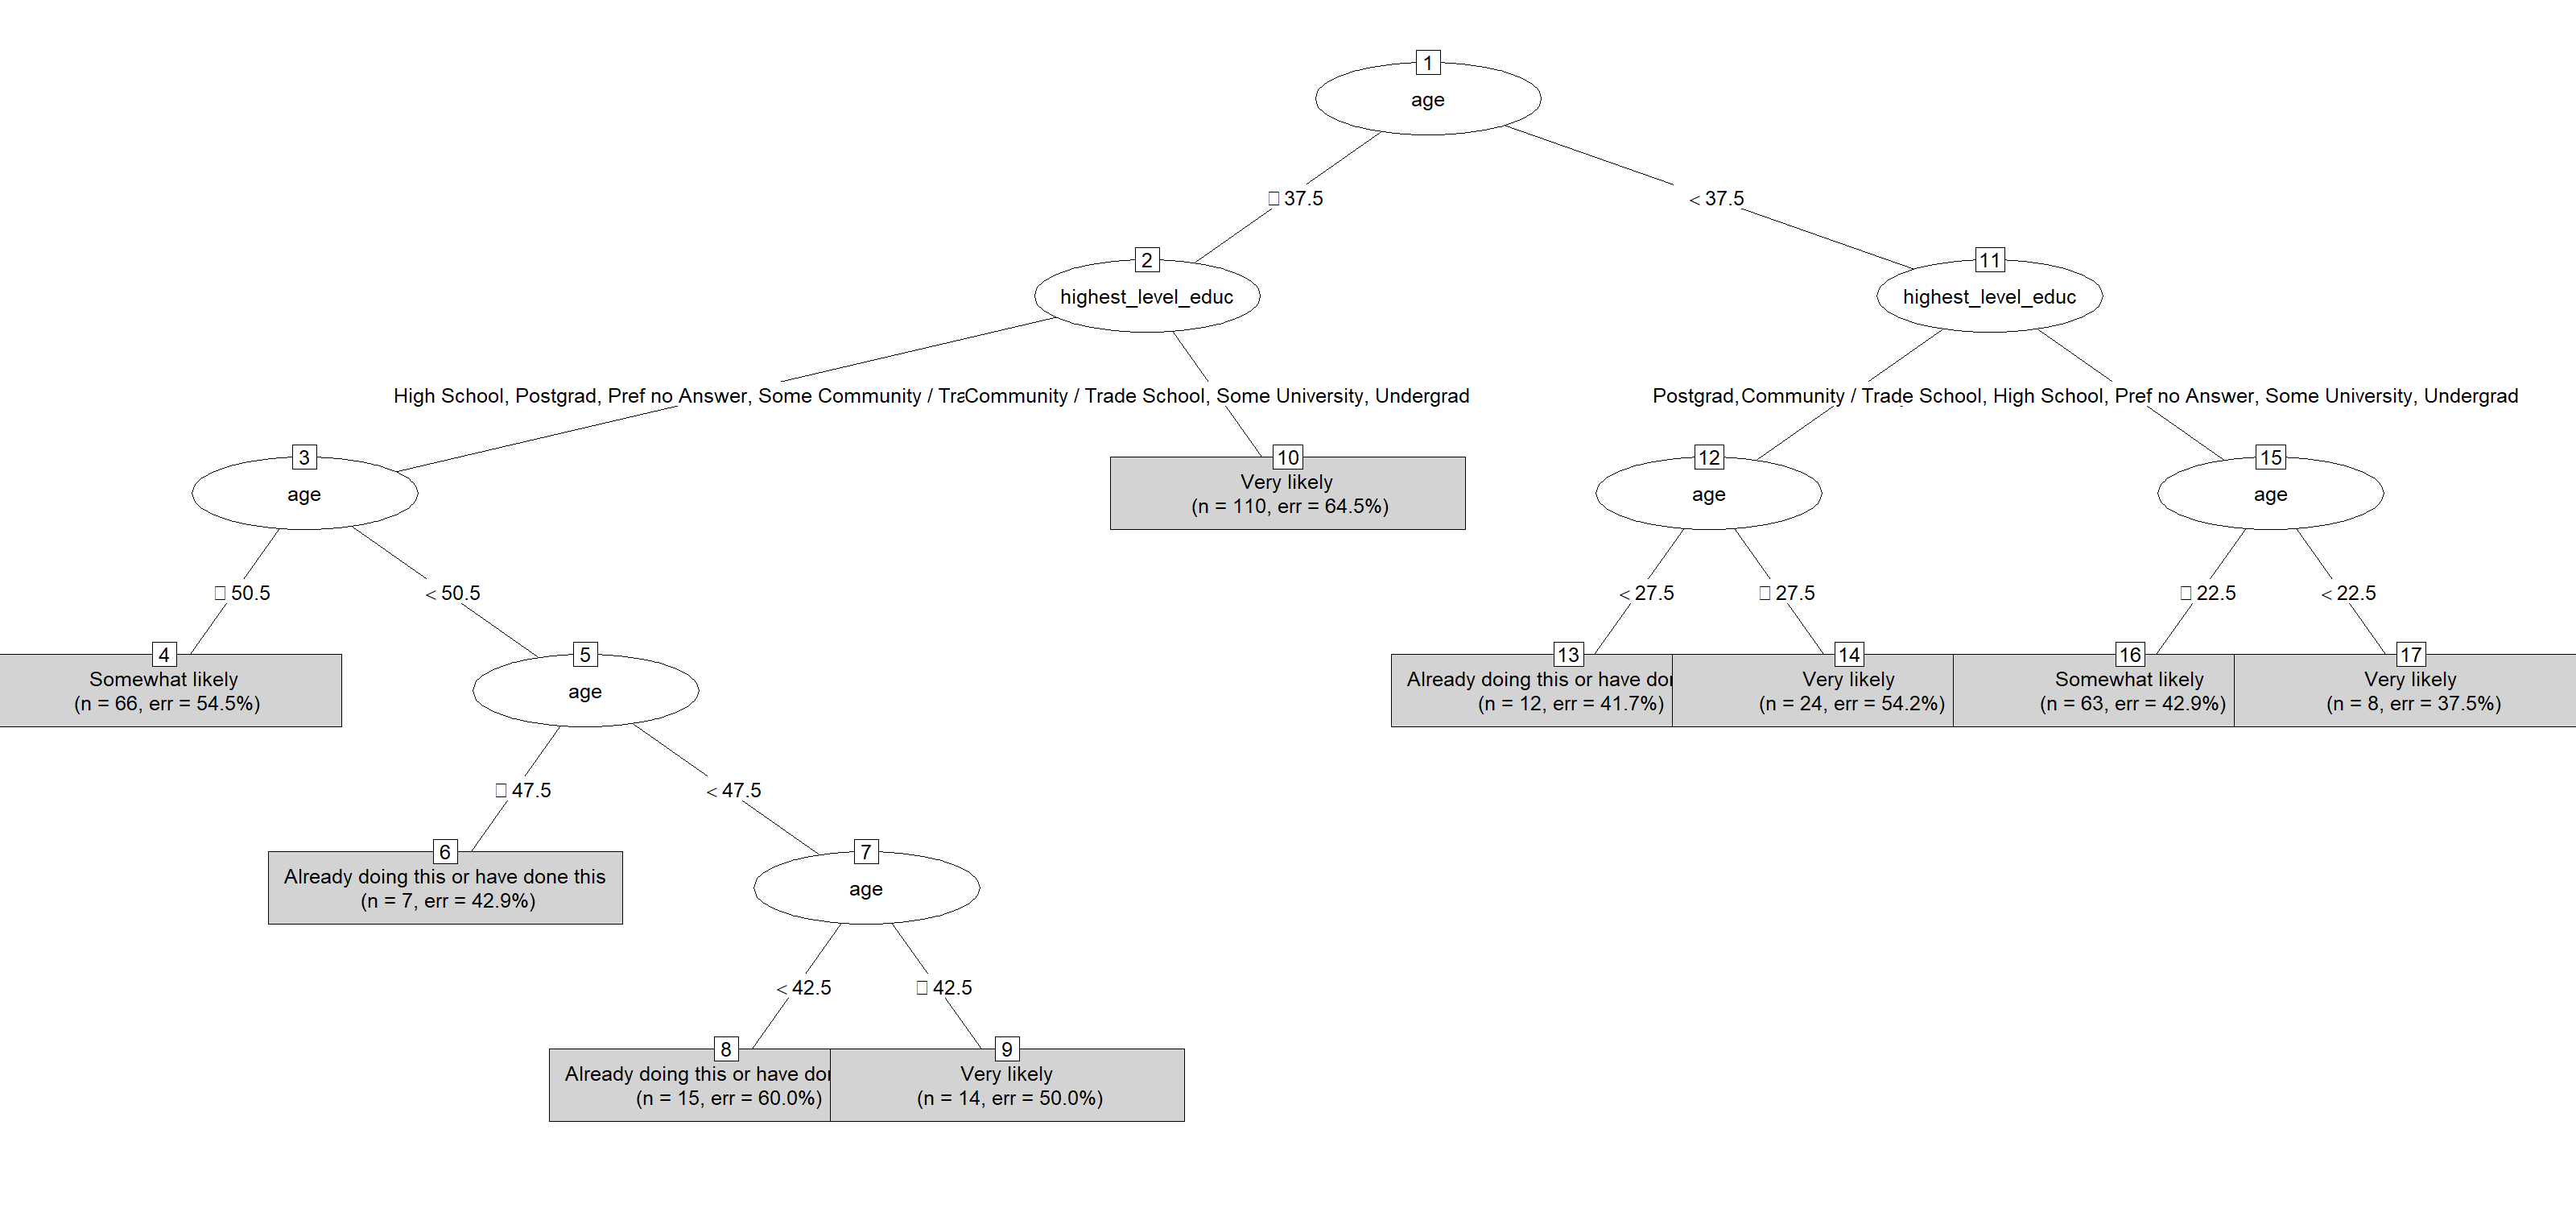
\includegraphics[width=10.67in,height=\textheight]{../data/04-model_data/green_product_tree.png}

}

\caption{Probability tree for likelihood of purchasing green products,
predicted by age and education.}

\end{figure}%

\subsubsection{Likelihood of reducing hydro
usage}\label{likelihood-of-reducing-hydro-usage}

\begin{figure}[H]

{\centering 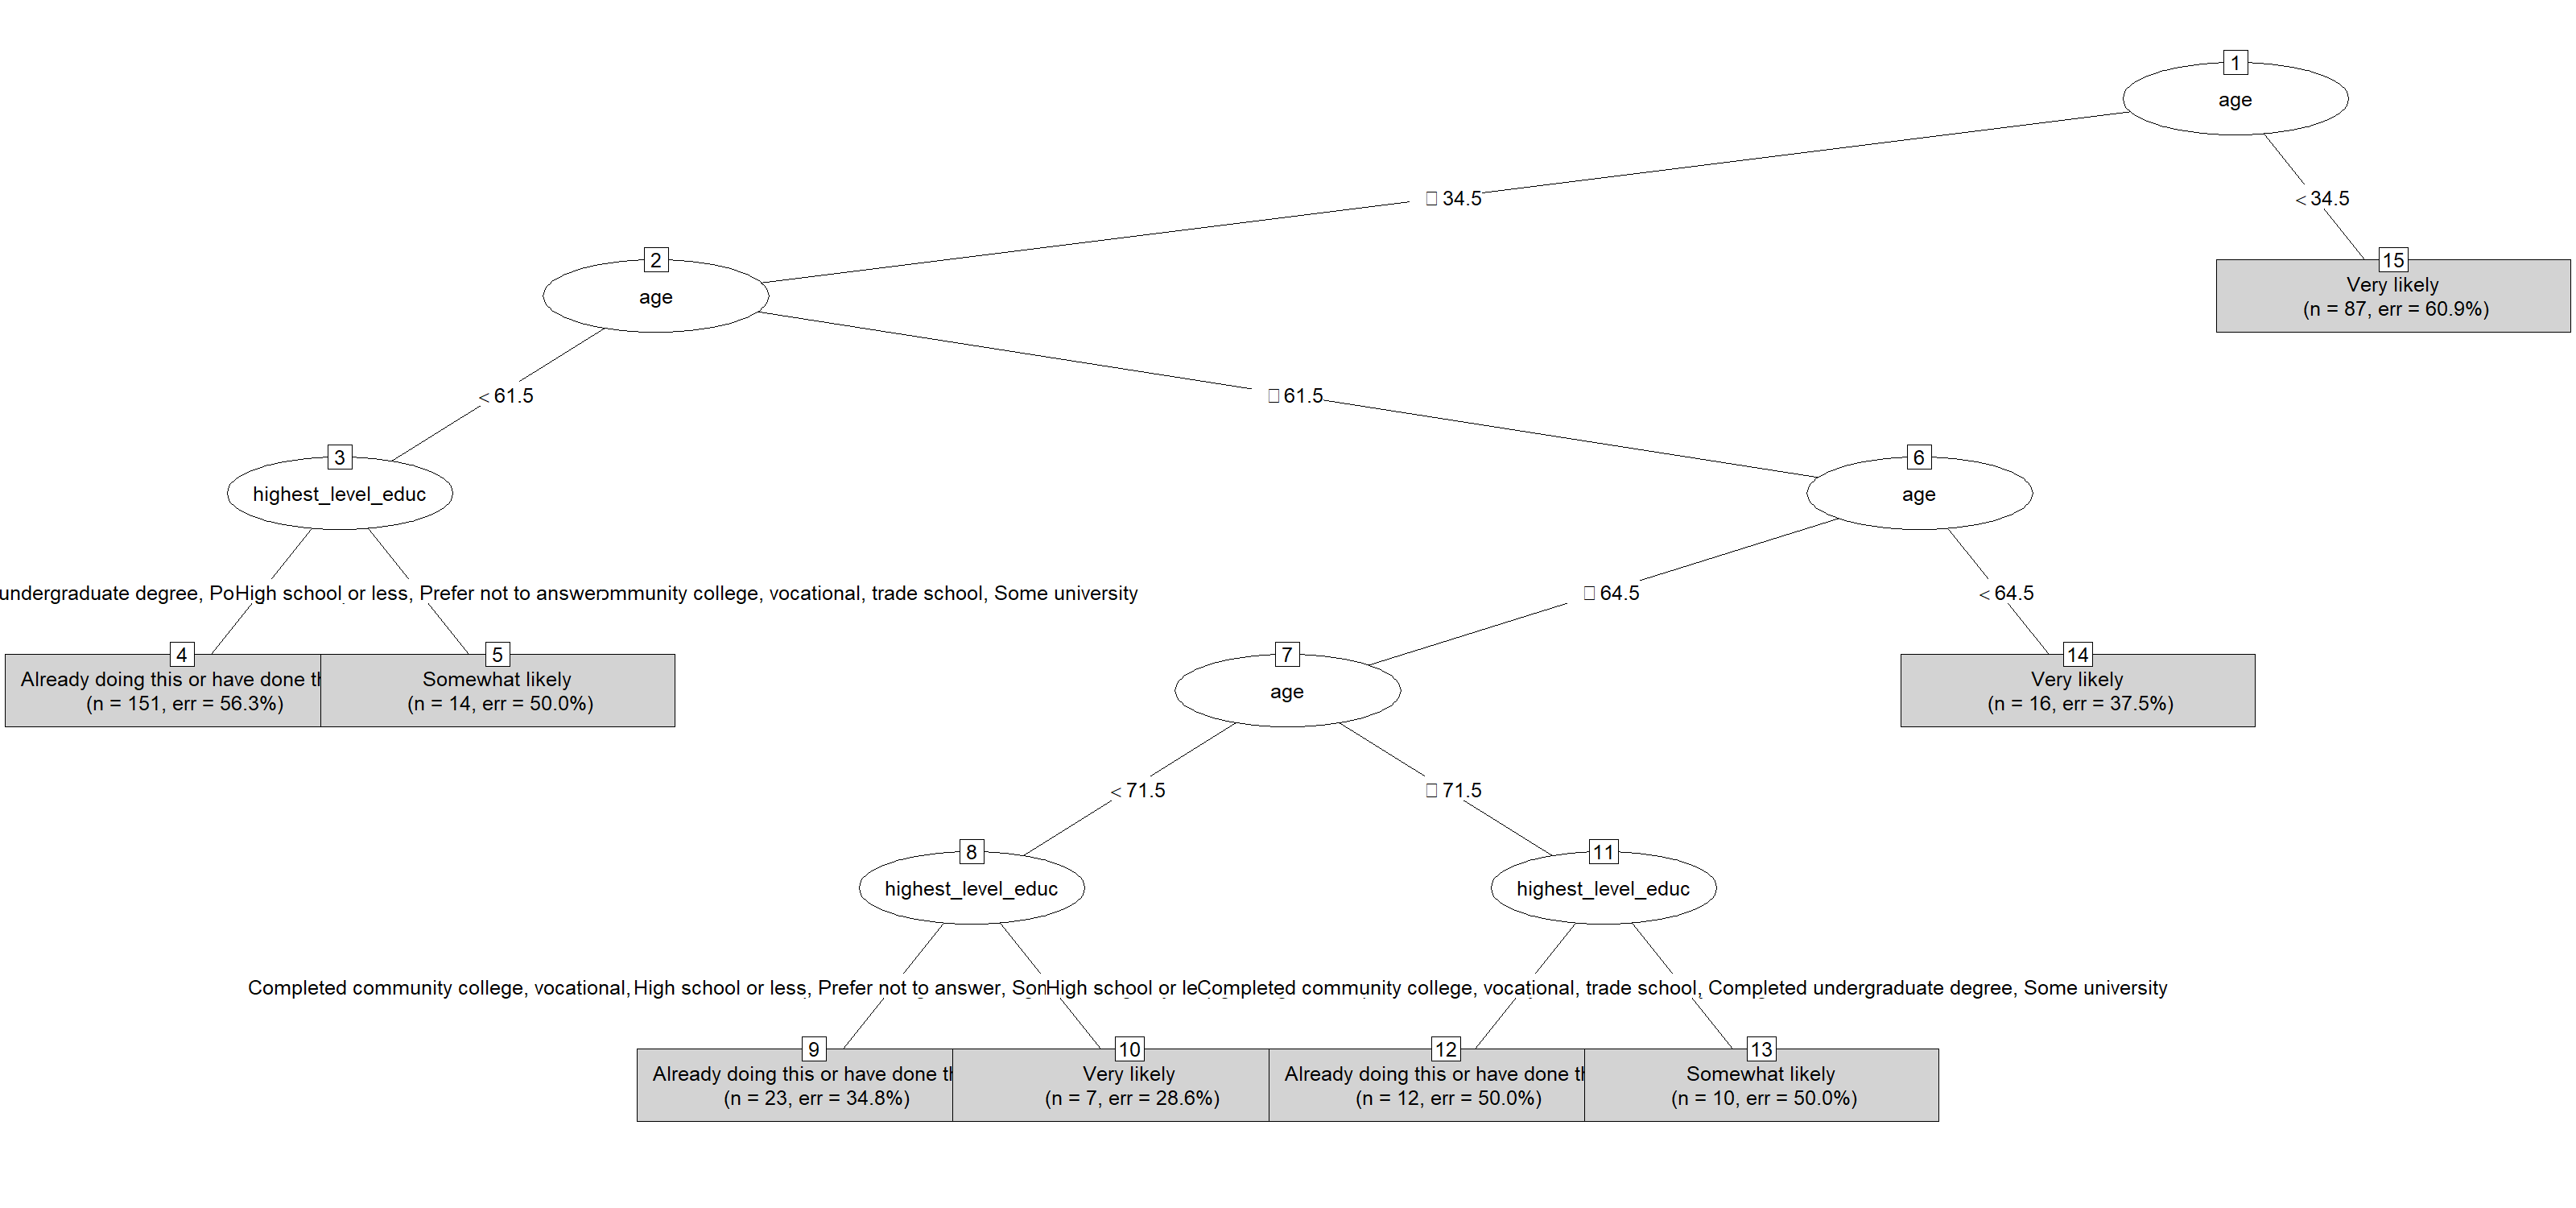
\includegraphics[width=10.67in,height=\textheight]{../data/04-model_data/reduce_hydro_tree.png}

}

\caption{Probability tree for likelihood of reducing hydro usage,
predicted by age and education.}

\end{figure}%

\subsubsection{Likelihood of reducing
waste}\label{likelihood-of-reducing-waste}

\begin{figure}[H]

{\centering 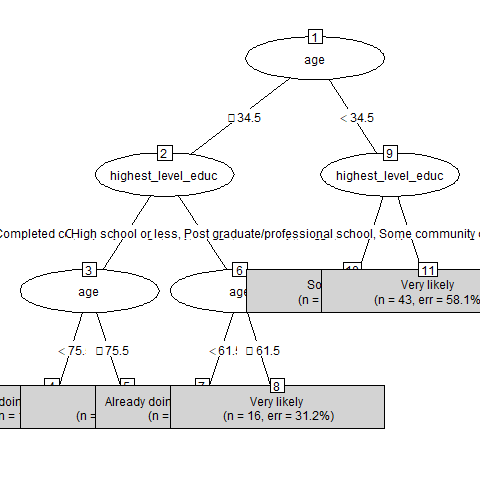
\includegraphics[width=10.67in,height=\textheight]{../data/04-model_data/reduce_waste_tree.png}

}

\caption{Probability tree for likelihood of reducing waste, predicted by
age and education.}

\end{figure}%

\subsubsection{Likelihood of sorting waste
correctly}\label{likelihood-of-sorting-waste-correctly}

\begin{figure}[H]

{\centering 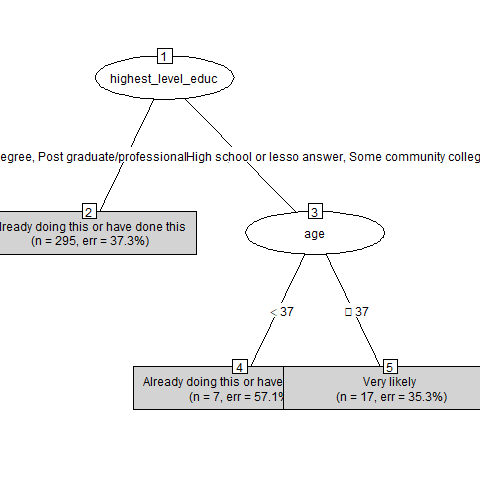
\includegraphics[width=10.67in,height=\textheight]{../data/04-model_data/sort_waste_tree.png}

}

\caption{Probability tree for likelihood of sorting waste correctly,
predicted by age and education.}

\end{figure}%

\subsubsection{Likelihood of walking or cycling shorter
distances}\label{likelihood-of-walking-or-cycling-shorter-distances}

\begin{figure}[H]

{\centering 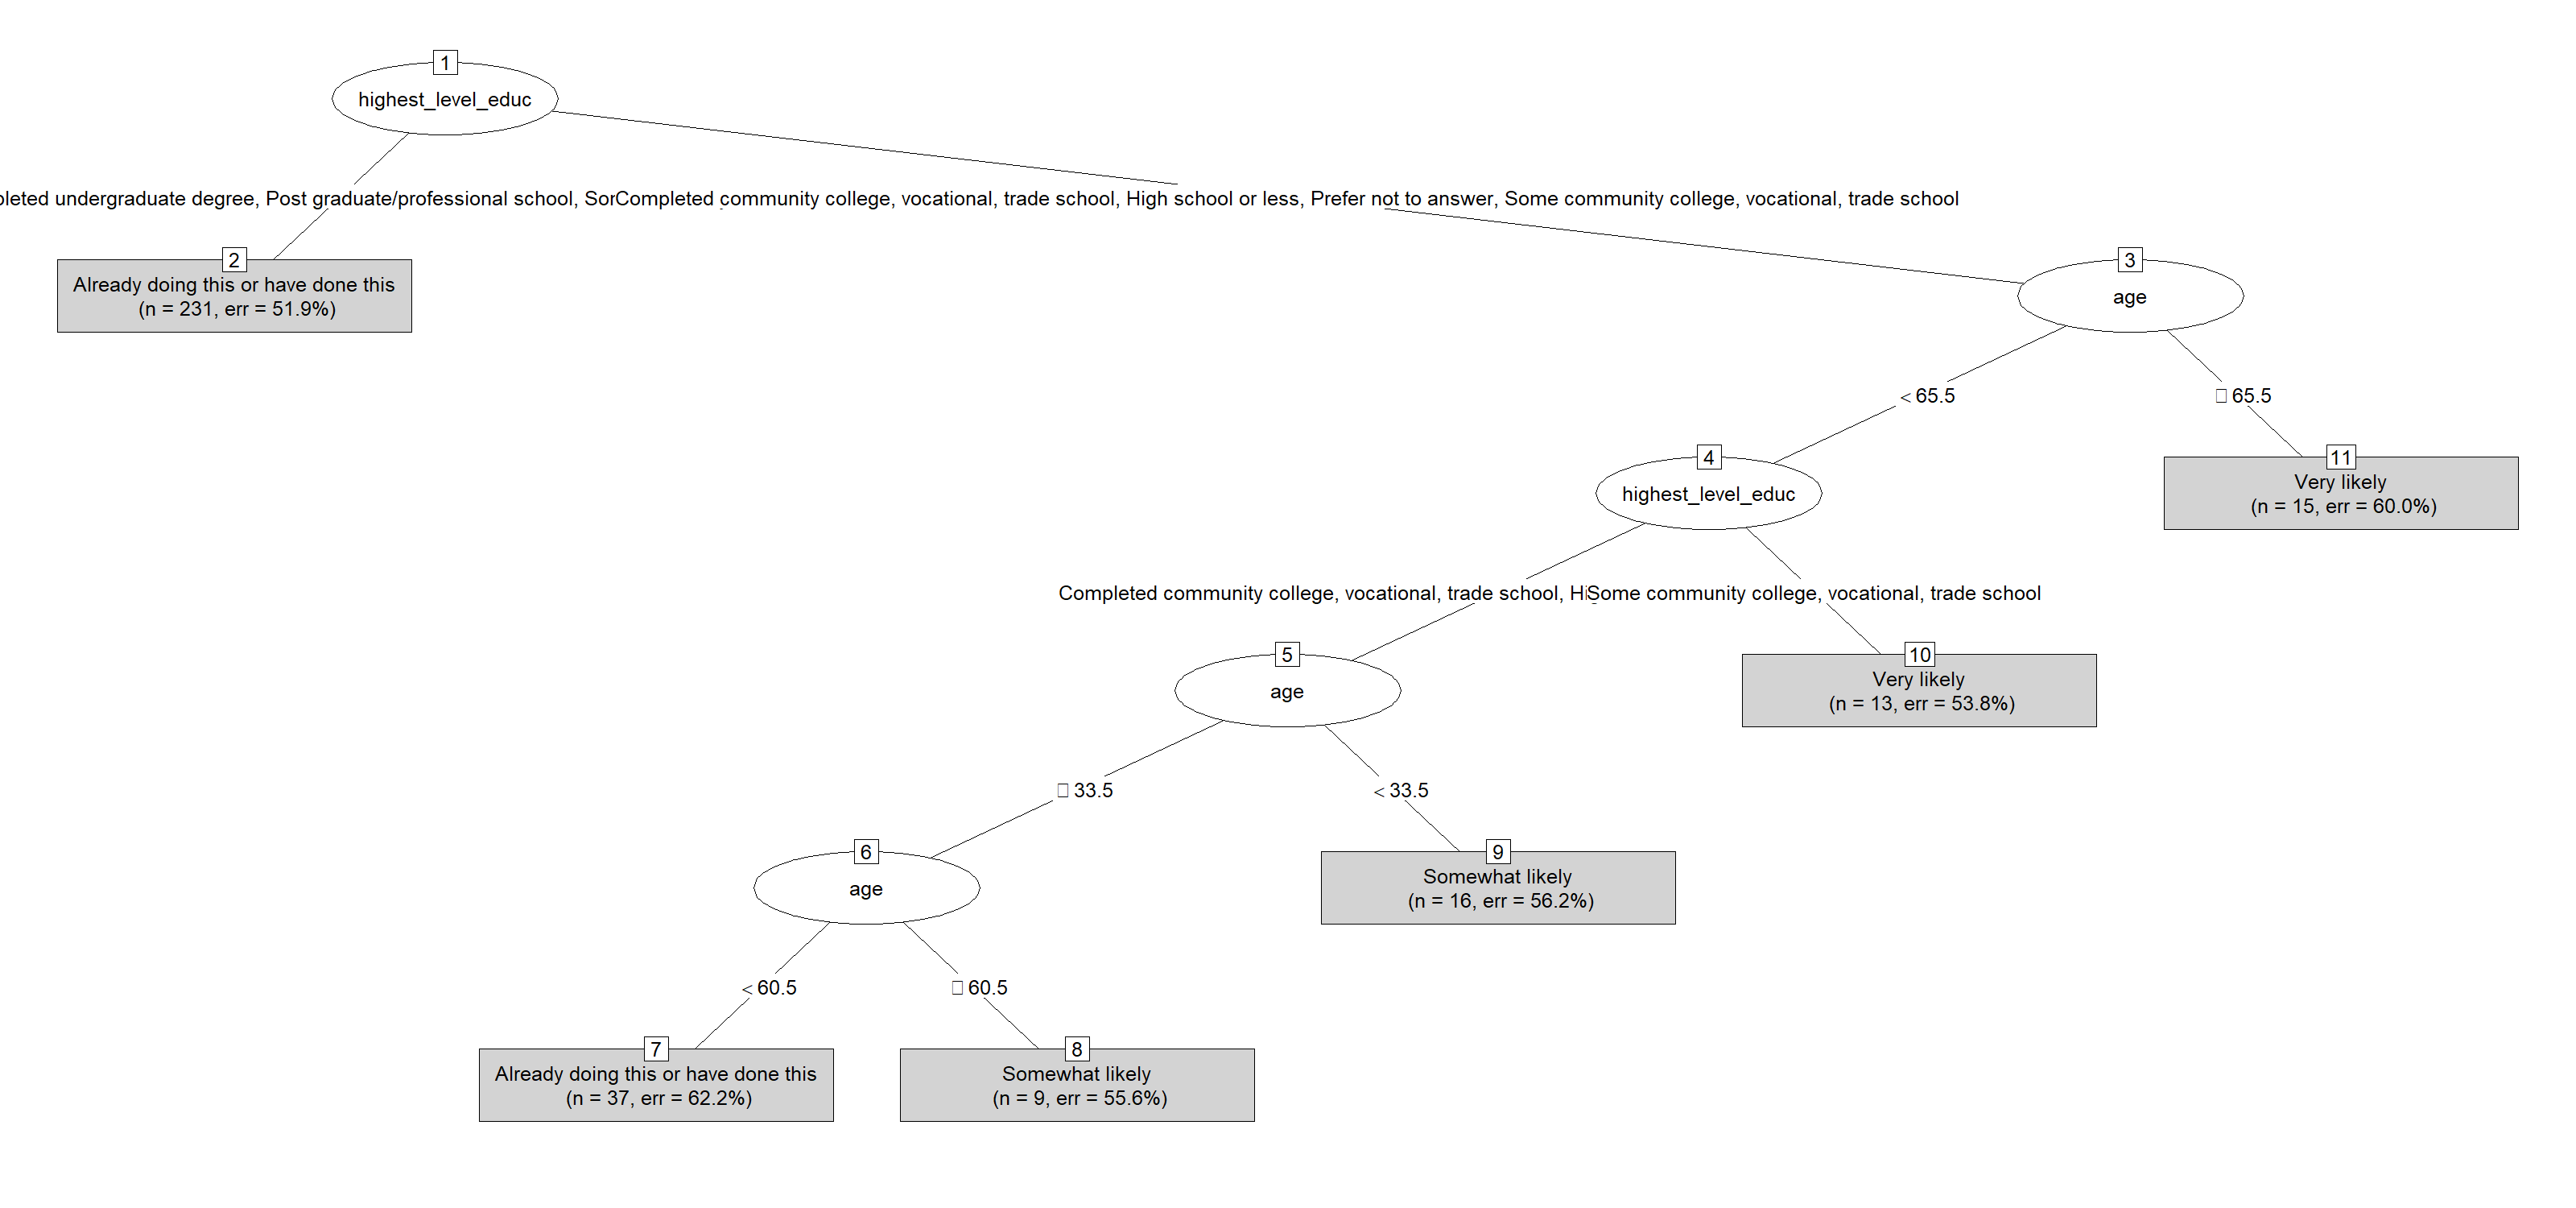
\includegraphics[width=10.67in,height=\textheight]{../data/04-model_data/short_distance_tree.png}

}

\caption{Probability tree for likelihood of walking or cycling shorter
distances, predicted by age and education.}

\end{figure}%

\subsection{Model Estimation and
Interpretation}\label{model-estimation-and-interpretation}

The probability tree model estimates how the predictors age and
education influence the likelihood of adopting climate-friendly
behaviors. By splitting the data into branches based on these variables,
the model helps identify decision rules that predict individuals'
likelihood of taking actions such as reducing waste or investing in
green products. We anticipate that younger individuals, due to greater
environmental awareness, are more likely to engage in climate-positive
actions, while those with higher levels of education may also be more
inclined to adopt such behaviors, given their increased awareness of
climate change and sustainable practices. The model estimates the
parameters for age and education using regression techniques, providing
coefficients that indicate how each factor influences the likelihood of
taking climate-friendly actions.

\section{Results}\label{results}

\subsection{Model Summary Table}\label{model-summary-table}

The table presents the accuracy of models predicting the likelihood of
various climate-friendly actions based on demographic factors such as
age and education. Each row represents a different climate action (e.g.,
home improvement, reducing hydro, minimizing car use), with the
corresponding accuracy of the model's predictions. The accuracy values
reflect how well the models, which use age and education as predictors,
align with the actual data. An accuracy of 33 percent for home
improvement'' indicates that the model correctly predicted the outcome
33\% of the time for this action. These accuracy values help evaluate
the effectiveness of age and education as predictors for each specific
climate action.

\begin{verbatim}
                Model Accuracy
1    home_improvement       33
2        reduce_hydro       28
3        minimize_car       39
4    vehicle_electric       25
5 protein_alternative       25
6        reduce_waste       39
\end{verbatim}

\subsection{Likelihood taking action by
age}\label{likelihood-taking-action-by-age}

Figure~\ref{fig-six} shows the relationship between age and the
likelihood of engaging in various climate-related actions. The x-axis
represents the age groups, and the y-axis indicates the percentage of
respondents reporting different likelihood levels, from ``Already doing
this'' to ``Very unlikely.'' The trend lines across each action show how
engagement varies by age.

\subsubsection{Electric / Hybrid Vehicle
Adoption}\label{electric-hybrid-vehicle-adoption}

Younger respondents (15-24, 25-34) are less likely to adopt electric or
hybrid vehicles, with only a small proportion already using or
considering them. Adoption rates increase slightly in the 55-64 age
group, then decline again in the 65+ group. This suggests that older
individuals may have more resources or stability to invest in electric
vehicles.

\subsubsection{Home Improvement for Energy
Efficiency}\label{home-improvement-for-energy-efficiency}

Middle-aged individuals (35-54) are the most likely to engage in home
improvement actions aimed at increasing energy efficiency. Younger age
groups (15-24, 25-34) report lower likelihoods, likely due to barriers
such as homeownership and disposable income.

\subsubsection{Consumption of Meat
Alternatives}\label{consumption-of-meat-alternatives}

Younger age groups, especially 15-24 and 25-34, are more likely to adopt
meat alternatives. As age increases, the likelihood of doing so
decreases, possibly due to established dietary habits in older
generations.

\subsubsection{Minimizing Car Use}\label{minimizing-car-use}

A trend similar to that of meat alternatives is observed, with younger
individuals more likely to minimize car use. Older respondents,
particularly those 65 and older, show less inclination to reduce car
usage, possibly due to mobility needs or lifestyle factors like suburban
living.

\subsubsection{Purchasing Green
Products}\label{purchasing-green-products}

The likelihood of purchasing green products is relatively uniform across
age groups. Middle-aged and older demographics show a slight increase in
engagement, but the trend line remains mostly flat, indicating that this
behavior is more influenced by factors such as income or environmental
awareness rather than age.

\subsubsection{Reducing Hydro Usage}\label{reducing-hydro-usage}

Older respondents (55-64 and 65+) are the most likely to reduce hydro
usage, likely driven by cost-saving measures or environmental concerns.
The trend line shows a steady increase with age.

\subsubsection{Reducing and Sorting
Waste}\label{reducing-and-sorting-waste}

Both reducing and sorting waste are more commonly reported by
middle-aged and older groups (45-64). This may reflect increased
awareness or resources for waste management.

\subsubsection{Walking / Cycling Short
Distances}\label{walking-cycling-short-distances}

Younger respondents (15-34) are more likely to engage in walking or
cycling short distances. As age increases, the likelihood of walking or
cycling decreases, possibly due to physical limitations or differing
lifestyle needs.

\begin{figure}

\centering{

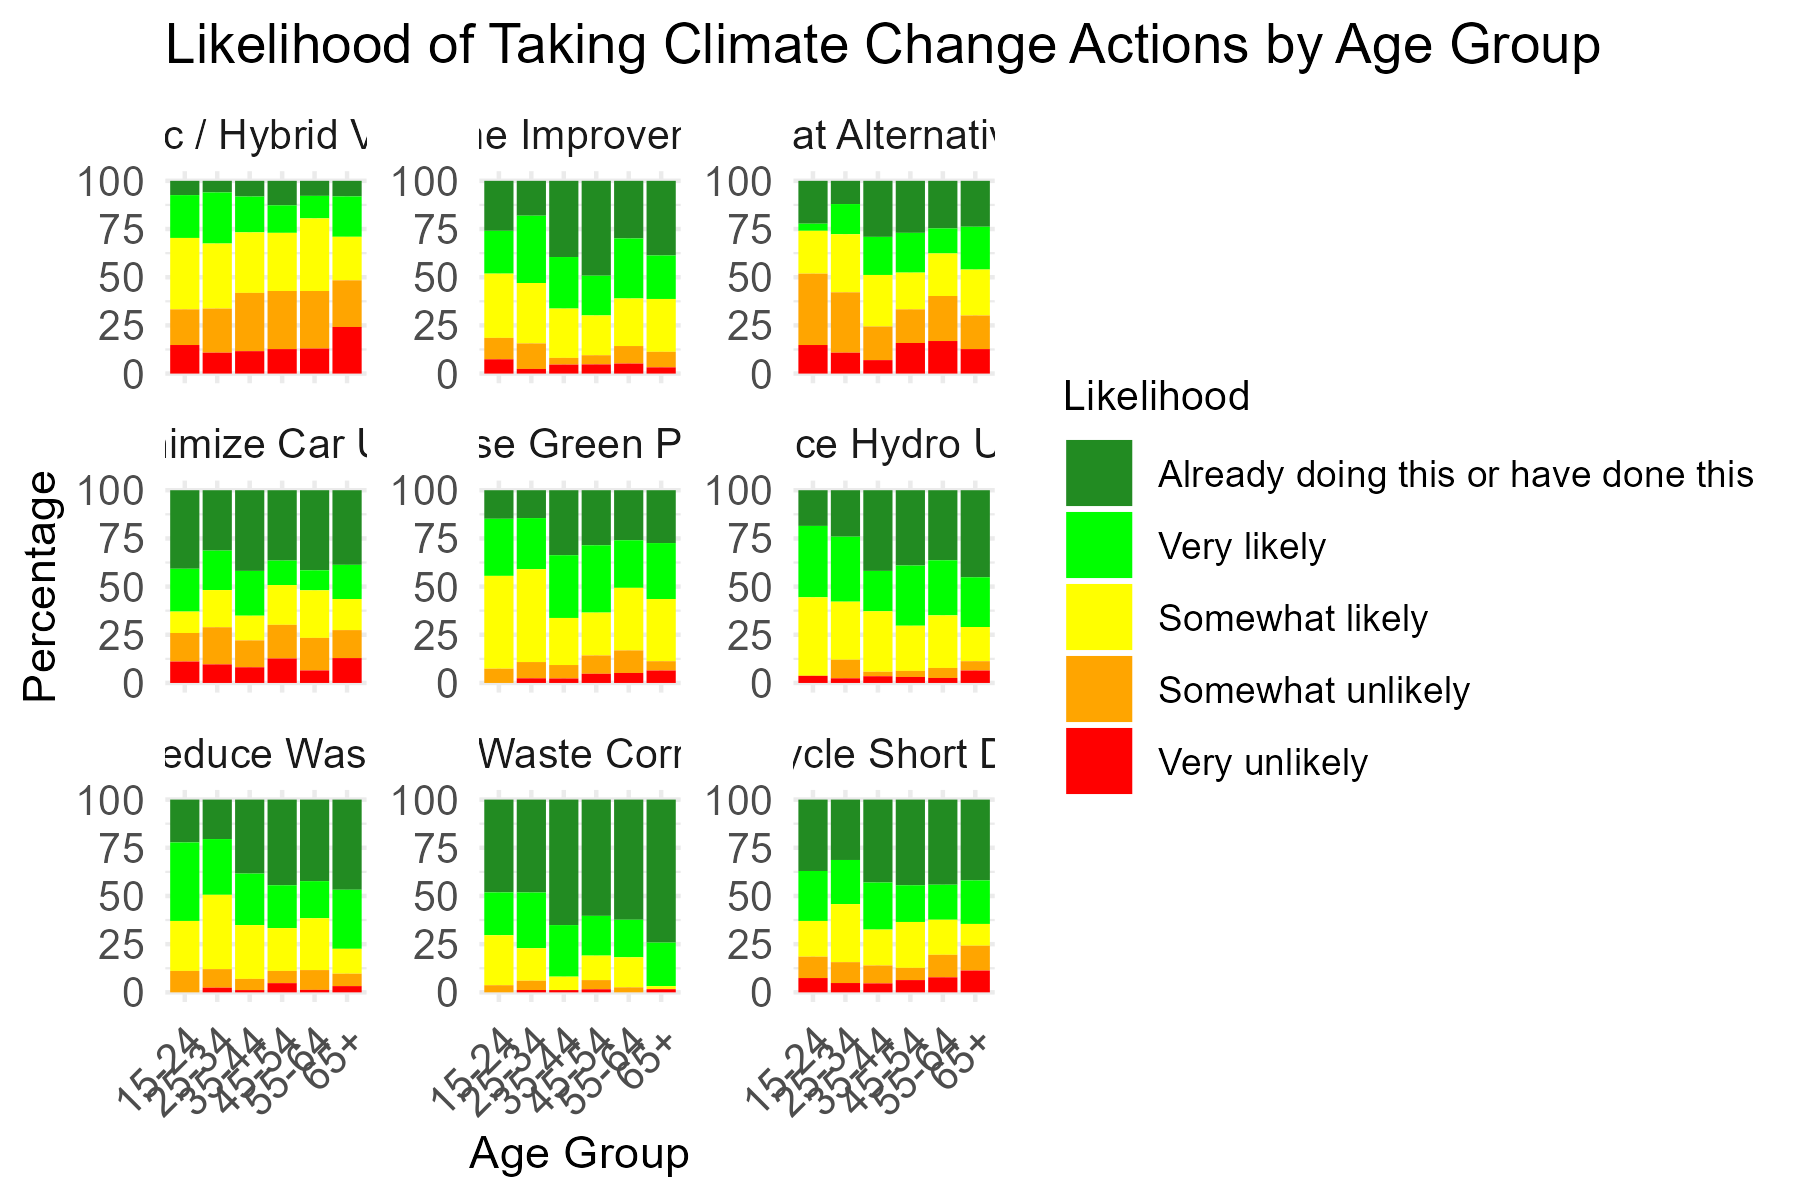
\includegraphics[width=6in,height=\textheight]{../data/03-figures_data/likelihood_age_plot.png}

}

\caption{\label{fig-six}Likelihood of Taking Climate Change Actions by
Age Group. The stacked bar chart illustrates the percentage of
respondents across six age groups (15-24, 25-34, 35-44, 45-54, 55-64,
65+) in terms of their self-reported likelihood to engage in nine
distinct climate-related actions. Each color represents a different
level of likelihood, from ``Already doing this or have done this'' to
``Very unlikely.'' The black dashed trend line highlights how the
likelihood of action changes across age groups, providing insights into
generational differences in climate-related behavior.}

\end{figure}%

\subsection{Likelihood taking action by
education}\label{likelihood-taking-action-by-education}

Figure~\ref{fig-seven} displays how the likelihood of engaging in
climate-friendly actions varies by educational attainment. The x-axis
represents the proportion of respondents in each education category,
while the y-axis lists the educational levels, from ``Prefer not to
answer'' to ``Postgrad.'' Each action is shown across separate facets,
revealing how education level correlates with engagement in each
behavior.

\subsubsection{Trends in Education Attainment and Climate-Friendly
Actions}\label{trends-in-education-attainment-and-climate-friendly-actions}

Individuals with higher education levels generally show a higher
likelihood of engaging in climate-friendly actions. This trend is
evident across all behaviors, with respondents possessing undergraduate
or postgraduate degrees more likely to adopt electric vehicles or
purchase green products.

\paragraph{Electric/Hybrid Vehicle
Adoption}\label{electrichybrid-vehicle-adoption}

Postgraduate degree holders are the most likely to have adopted or
consider adopting electric or hybrid vehicles. In contrast, respondents
with lower education levels, such as those with high school or less, are
more likely to report being ``Very unlikely'' or ``Somewhat unlikely''
to adopt these vehicles.

\paragraph{Minimizing Car Use}\label{minimizing-car-use-1}

Higher education levels correlate with a greater likelihood of
minimizing car use, though the trend is less pronounced for individuals
with lower education levels.

\paragraph{Reducing Hydro Usage}\label{reducing-hydro-usage-1}

While education has a smaller impact on reducing hydro usage compared to
other actions, those with higher education levels are still more likely
to engage in this behavior.

\paragraph{Purchasing Green Products and Reducing
Waste}\label{purchasing-green-products-and-reducing-waste}

Purchasing green products and reducing waste are more common among
individuals with postsecondary education, especially those with
undergraduate or postgraduate degrees. In contrast, individuals with
lower education levels report more moderate engagement with these
actions.

\subsubsection{Adopting Meat
Alternatives}\label{adopting-meat-alternatives}

Higher education is associated with greater adoption of meat
alternatives. This is particularly true for those with undergraduate or
postgraduate education, while fewer respondents with lower education
levels report engaging in this behavior.

\subsubsection{Walking or Cycling Short
Distances}\label{walking-or-cycling-short-distances}

Walking or cycling short distances is a behavior that is relatively
common across all education levels, though individuals with higher
education levels show slightly higher engagement.

\subsubsection{Sorting Waste Correctly}\label{sorting-waste-correctly}

Sorting waste correctly is one of the most consistently adopted
behaviors across all education levels, with a relatively small
proportion of respondents indicating they are unlikely to engage in this
action. However, individuals with higher education are still more likely
to fall in the ``Already doing this'' category.

\begin{figure}

\centering{

\captionsetup{labelsep=none}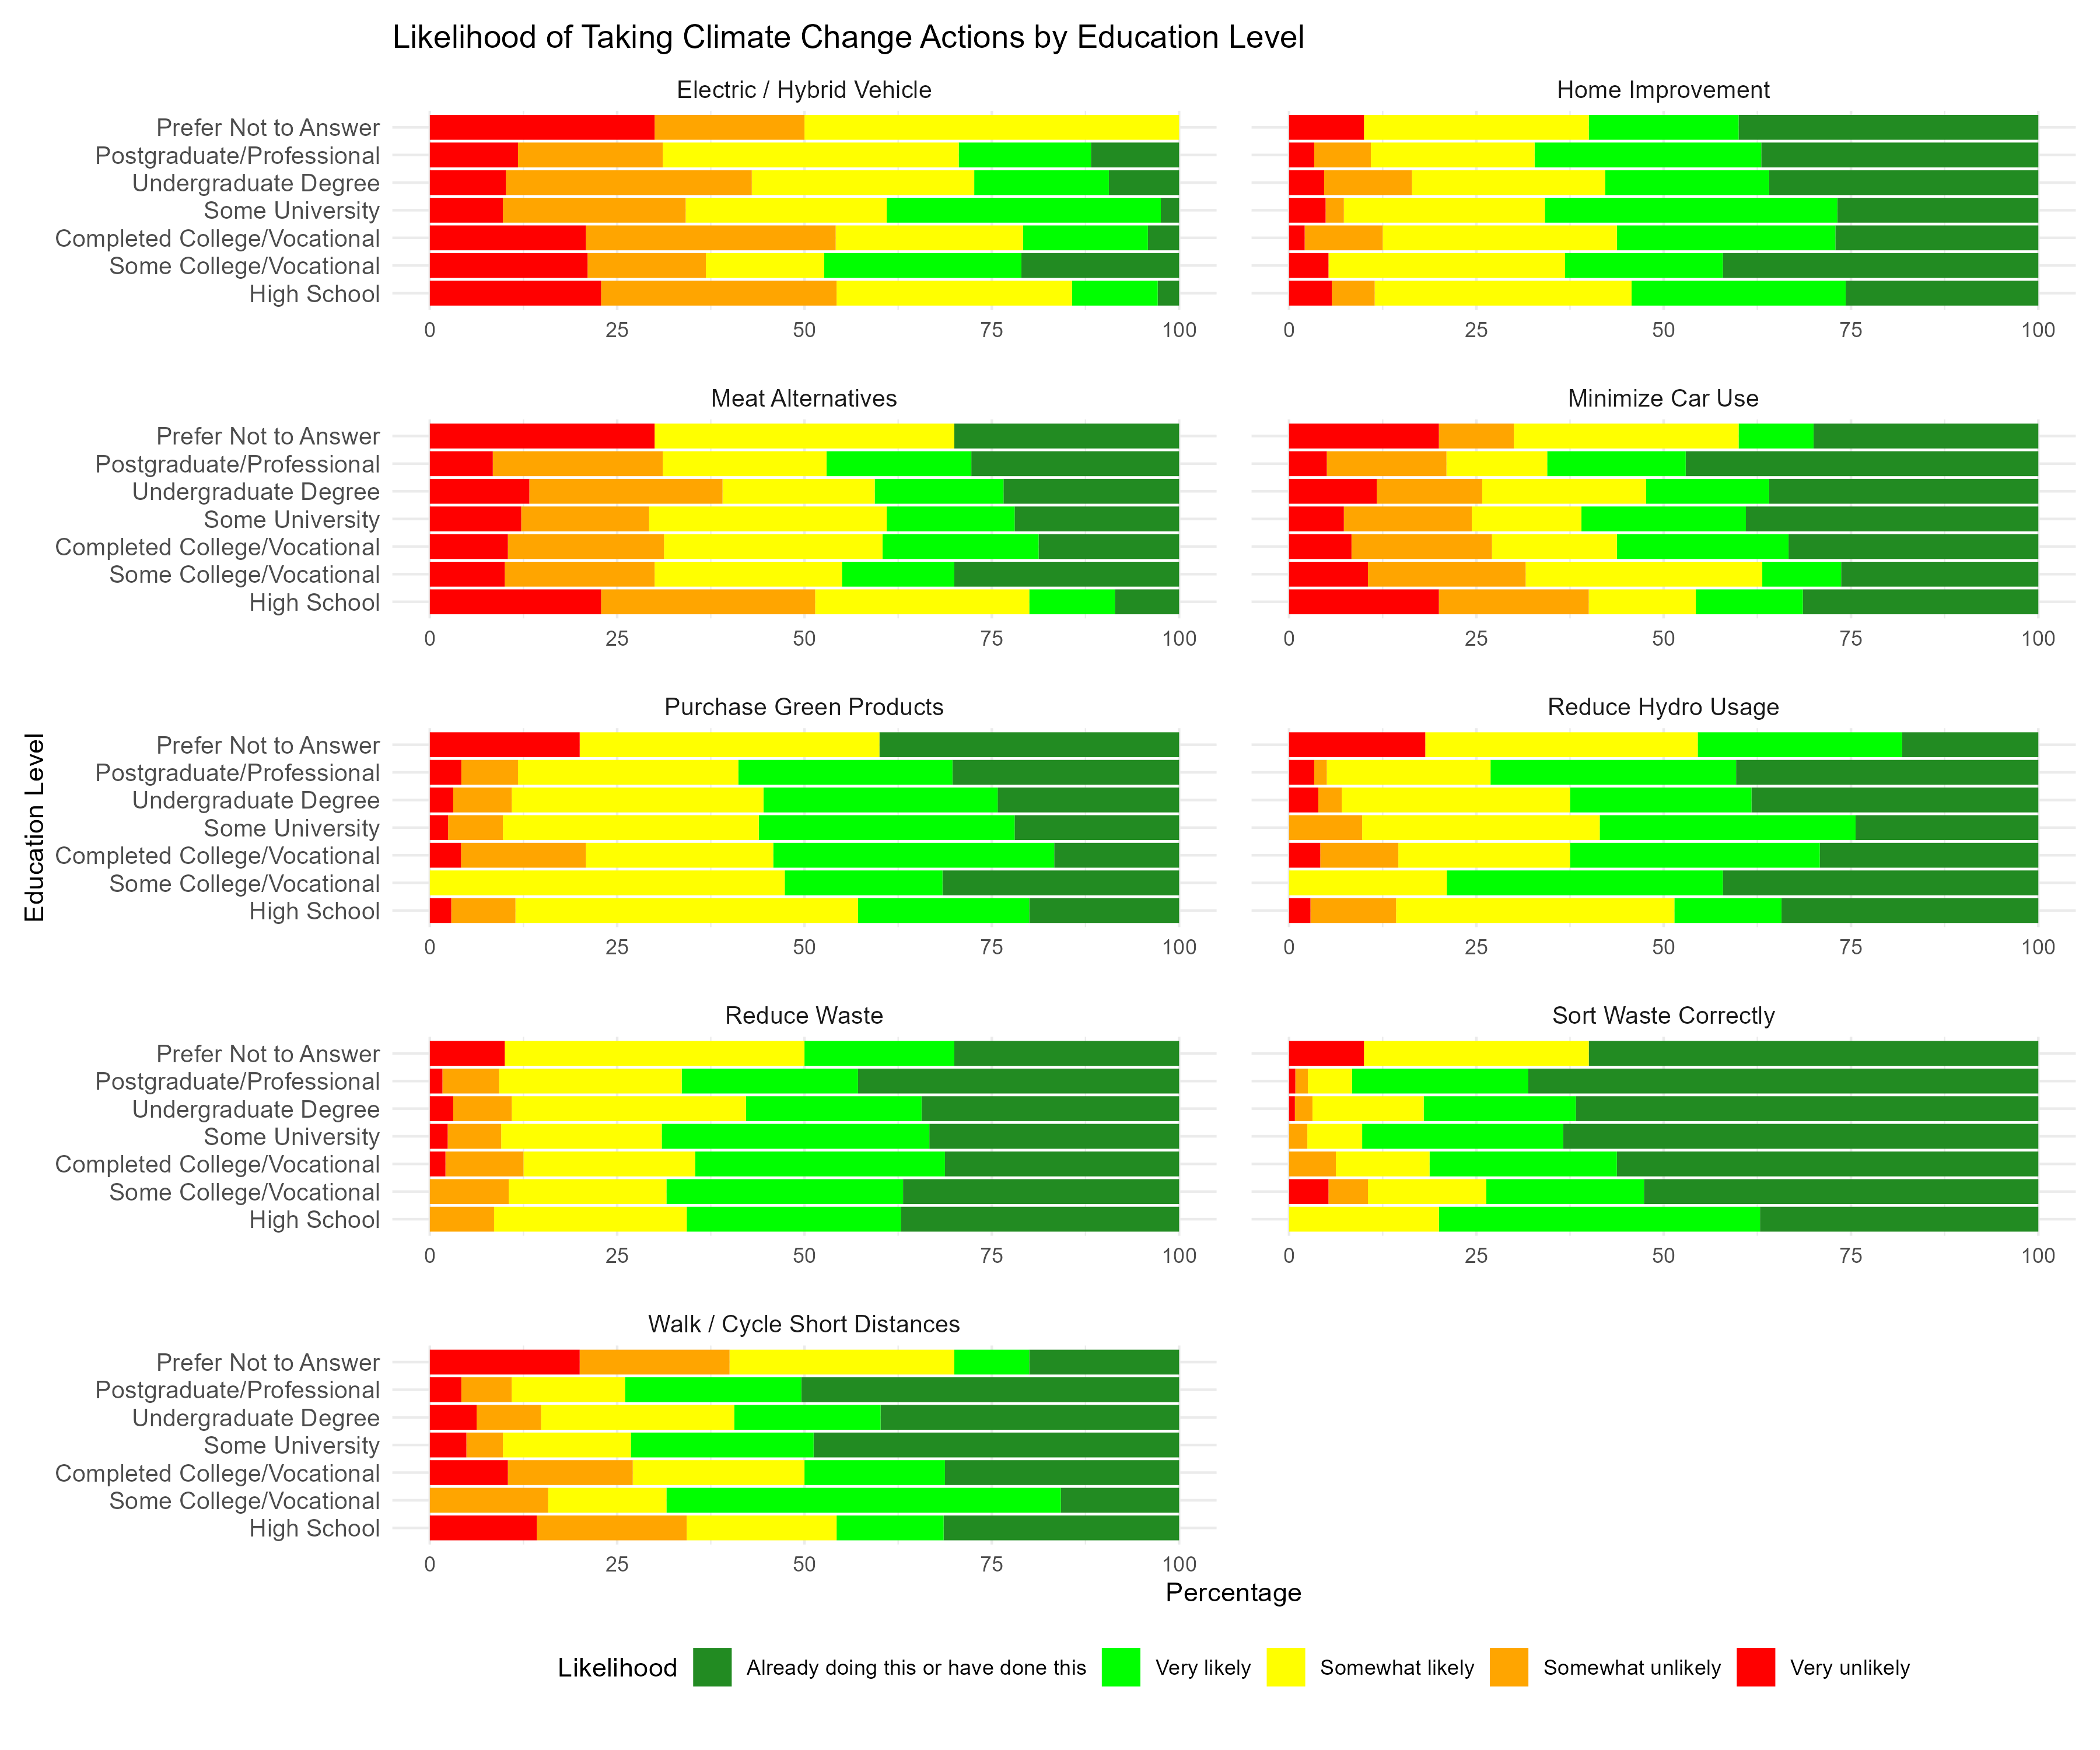
\includegraphics[width=6in,height=\textheight]{../data/03-figures_data/likelihood_education_plot.png}

}

\caption{\label{fig-seven}}

\end{figure}%

\subsection{Overall Summary of
Results:}\label{overall-summary-of-results}

The results indicate that both age and education significantly influence
the likelihood of engaging in climate-related actions. Younger
respondents tend to be more likely to adopt behaviors such as consuming
meat alternatives and minimizing car use, while older individuals are
more inclined to engage in actions that require larger investments or
long-term commitments, such as reducing hydro usage and investing in
energy-efficient home improvements. Higher educational attainment is
also strongly linked to a greater likelihood of engaging in
climate-friendly behaviors, particularly those that involve financial
investment, like adopting electric vehicles and consuming meat
alternatives. However, simpler actions such as sorting waste correctly
are more widely reported across all education levels. These generational
and educational differences highlight the importance of factors such as
income, lifestyle, and environmental awareness in shaping individuals'
climate-related behaviors. In light of these findings, it is crucial to
consider demographic factors when designing policies or campaigns aimed
at encouraging climate action, as different age and education groups
exhibit varied levels of engagement with both simple and more complex
sustainable practices.

\section{Discussion}\label{discussion}

\subsection{Age and Climate-Friendly Behaviors}\label{sec-first-point}

The findings indicate that younger individuals are more likely to engage
in climate-friendly actions perceived as low-cost and easier to
implement, such as consuming meat alternatives and reducing car usage.
The model results show that these behaviors have relatively higher
predicted likelihoods among younger participants, aligning with existing
research on generational differences in environmental attitudes. This
trend may be driven by heightened environmental awareness and increased
exposure to climate change discussions among younger generations, often
through social media and educational initiatives. These results suggest
that lifestyle factors and generational attitudes significantly shape
behavioral patterns, with younger individuals gravitating toward actions
that are both socially encouraged and accessible.

\subsection{The Role of Education in Sustainable
Actions}\label{sec-second-point}

Education significantly influences individuals' likelihood of engaging
in more substantial climate-friendly behaviors. Our models demonstrate
that individuals with higher educational attainment are more likely to
adopt behaviors requiring greater financial or logistical investment,
such as purchasing electric vehicles or making energy-efficient home
improvements. The accuracy of the models predicting these behaviors is
relatively lower than for simpler actions, suggesting that education is
an important but not sole determinant. This relationship between
education and sustainability underscores the importance of knowledge and
informed decision-making in supporting climate-friendly actions,
particularly those with long-term environmental benefits. The data
suggests that higher education increases both environmental awareness
and the capacity to implement financially demanding sustainable
practices, which are often inaccessible to those with lower educational
levels.

\subsection{The Influence of Climate Change
Knowledge}\label{sec-third-point}

Self-reported knowledge of climate change also plays a role in the
likelihood of adopting sustainable behaviors. Our analysis shows that
individuals with greater awareness are more proactive in making
environmentally conscious choices, particularly for actions like
reducing waste and conserving energy. However, the model accuracy for
some knowledge-based behaviors remains moderate, highlighting a gap
between awareness and action. This suggests that while raising awareness
is critical, it must be paired with policies that reduce structural
barriers to adopting more expensive or long-term sustainable actions.
For example, financial incentives or subsidies for purchasing
energy-efficient appliances could bridge this gap, ensuring individuals
are both informed and able to make practical changes.

\subsection{Limitations}\label{limitations}

One significant limitation of this study is its reliance on
self-reported survey data, which is inherently prone to biases such as
social desirability bias and recall errors. Respondents may overestimate
their environmental knowledge or exaggerate their participation in
climate-friendly behaviors to present themselves in a favorable light.
This introduces uncertainty into the accuracy of the models, as the
input data may not fully reflect actual behaviors or knowledge levels.
Additionally, self-reported data often lacks the granularity needed to
explore complex interactions between socio-economic factors, such as
income and household size, which can significantly influence sustainable
actions.

Another limitation arises from the use of summary data from the 2018 and
2021 surveys instead of individual-level data. While the summary
statistics provided valuable insights into broad demographic trends,
they limited the study's ability to explore more nuanced patterns and
interactions. For example, the summary data showed differences in
education and age trends between 2018 and 2021, but without
individual-level data, it was difficult to determine the direct effect
of socio-economic factors on climate action likelihood. Future studies
with access to raw, individual-level data could offer more precise
estimates and a deeper understanding of these dynamics.

\subsection{Challenges with Survey
Data}\label{challenges-with-survey-data}

Survey data presents additional challenges, such as non-response bias,
where certain demographic groups may be underrepresented, leading to
skewed results. Additionally, the framing of survey questions can
influence how respondents perceive and answer them, introducing further
variability in the data. The inability to verify self-reported behaviors
also limits the reliability of the conclusions drawn from such datasets.
Despite these challenges, surveys remain a valuable tool for capturing
perceptions and self-reported behaviors, but their findings should be
interpreted with caution and, when possible, supplemented with objective
data sources.

\subsection{Future Directions}\label{future-directions}

Future research should aim to identify the specific barriers preventing
certain demographic groups from adopting climate-friendly behaviors.
This could involve examining factors such as income, access to
resources, and perceived obstacles to sustainable practices.
Additionally, targeted interventions, such as financial subsidies,
public awareness campaigns, or infrastructure improvements, could make
sustainable actions more accessible and affordable. Longitudinal studies
would be particularly valuable for tracking how awareness of climate
change influences sustained behavioral changes over time. Comparing
individual-level data across different years could also provide insights
into the long-term impact of educational and policy interventions on
climate-friendly behaviors.

Lastly, integrating objective data, such as energy consumption records
or transportation usage statistics, could validate and enhance the
accuracy of survey-based findings. This combined approach would offer a
more comprehensive understanding of how demographic and socio-economic
factors influence the adoption of sustainable actions, ultimately
informing more effective climate policies and interventions.

\section{Conclusion}\label{sec-conclusion}

This study provides valuable insights into the demographic factors that
influence individuals' likelihood to engage in climate-friendly
behaviors, particularly age, education, and climate change knowledge.
Younger individuals and those with higher levels of education are more
likely to adopt sustainable behaviors, particularly those that require
greater financial investment or long-term commitment. However, barriers
such as financial constraints and access to resources remain significant
challenges. Addressing these barriers through targeted policies and
interventions could help make sustainable behaviors more accessible and
the norm across all demographic groups. Future research should explore
the underlying reasons for resistance to adopting climate-friendly
behaviors and how external factors can help overcome these challenges to
achieve widespread climate action.

\newpage

\appendix

\section{Appendix}\label{sec-appendix}

\section{Idealized methodology}\label{sec-idealized-meth}

\subsection{Survey objectives}\label{survey-objectives}

The primary objective of this study is to explore the factors
influencing the likelihood of individuals engaging in climate-friendly
behaviors. Specifically, the study aims to identify the age groups that
are least likely to participate in sustainable actions and investigate
how education levels impact climate-friendly behaviors. The research
also seeks to determine whether individuals who report being relatively
informed about climate change causes are more likely to take action to
mitigate it. The underlying assumption is that individuals with greater
knowledge of climate change should be more inclined to adopt behaviors
that reduce its impact. Additionally, the study will examine the
barriers that prevent people from engaging in sustainable behaviors,
with the goal of identifying strategies to make these actions more
accessible, affordable, and easy to adopt. The overarching aim is to
develop solutions to increase the likelihood of participation in
climate-friendly behaviors by removing existing barriers and promoting
sustainability across different demographic groups. Part of this
involves determining the most effective platforms for disseminating
information about climate change, specifically by identifying which
communication methods resonate most with different age groups. The
research will also explore the role of education systems in fostering
climate awareness and encouraging sustainable actions from a young age.
Ultimately, the findings aim to provide actionable solutions to promote
wider participation in climate-friendly actions, contributing to the
fight against climate change.

\subsection{Sampling approach}\label{sampling-approach}

This study will target a diverse set of respondents across various age
groups and demographic characteristics to gain a comprehensive
understanding of climate-friendly behaviors and their drivers. The
sample will be stratified to ensure representation across youth and
adult demographics, enabling a comparison of climate knowledge and
behaviors between generations. The study will start by sampling youth as
young as age 12. This age group is chosen because children are old
enough to understand the basics of climate change and the actions
required to address it but still impressionable enough for their
behaviors to be influenced by education and social interventions. By
including participants starting at age 12, we aim to assess how
effective climate change education in schools is and whether it is
shaping climate-friendly behaviors in the younger generation.

In addition to youth, adults aged 18 and older will also be included to
provide insight into longer-term behavioral trends, which may have been
shaped by earlier education or a lack of education on the subject. The
sampling will be stratified according to age, education level, income,
and geographic location to capture a broad spectrum of experiences and
perspectives on climate change and sustainability. Age groups will be
divided into the following ranges: 12-17, 18-24, 25-34, 35-44, 45-54,
55-64, and 65+, while education levels will range from middle school to
postgraduate education. Income will be categorized as low
(\textless\$30,000), middle (\$30,000--\$99,999), and high
(\textgreater\$100,000), and participants will also be grouped based on
urban, suburban, or rural geographic locations. This stratified sampling
approach ensures a diverse representation of individuals, allowing for
meaningful comparisons of climate knowledge and behaviors across
different demographic groups.

\subsection{Respondant recruitment}\label{respondant-recruitment}

Participants will be recruited using a multi-channel approach to ensure
broad representation across various age groups and geographic locations.
For youth aged 12-17, recruitment will occur through schools, with
cooperation from middle and high schools. District educational boards or
individual teachers will be approached to distribute information about
the survey, and parental consent will be obtained before participation.
To recruit adults, online surveys will be distributed via social media,
email lists, and relevant climate-focused online communities.
Additionally, outreach will be conducted in community centers and public
spaces to capture respondents from rural or underserved areas. Flyers,
local advertisements, and community events will help ensure that the
sample is representative of both urban and rural populations.

Incentives such as gift cards or a donation to a climate-focused charity
will be offered to participants to encourage engagement and improve
response rates, especially among younger participants who may be less
inclined to participate without an incentive.

\subsection{Data Validation}\label{data-validation}

To ensure the validity and reliability of the data, several validation
mechanisms will be employed. Responses will be reviewed for internal
consistency, such as cross-checking whether respondents who claim high
levels of climate change knowledge also report engaging in corresponding
climate-friendly behaviors. Participants who provide inconsistent
answers or fail to complete the survey will be excluded from the
analysis. Additionally, respondents may be contacted for clarification
if their answers are ambiguous or incomplete. This will ensure that the
data accurately reflects the participant's true attitudes and behaviors.

\section{Weighting and Data
adjustments}\label{weighting-and-data-adjustments}

The data collected will be weighted to account for any imbalances in
demographic representation within the sample. Statistical weighting will
adjust for factors such as age, education level, income, and geographic
location to ensure the sample accurately reflects the broader
population. Weighting will correct for any over- or under-representation
of specific demographic groups, allowing for more generalizable
findings. Additionally, data will be adjusted for non-response bias,
with greater weight given to underrepresented groups (e.g., certain age
groups or income levels) to correct for gaps in participation.

\subsection{Budget}\label{budget}

The budget for this study will cover several key areas essential for
effective data collection and analysis. A portion of the budget will be
allocated to the survey platform and software tools needed for data
collection, such as online survey tools and platforms for both youth and
adult respondents. Since incentives are critical to encouraging
participation, especially from younger individuals, funds will also be
used to provide gift cards or donations to climate-related charities as
incentives. To reach a diverse demographic, outreach costs will also be
factored in, including the production and distribution of flyers, local
advertisements, and outreach at community centers or schools. Lastly,
resources will be dedicated to data analysis, including the purchase of
statistical software like SPSS or R for cleaning, coding, and analyzing
the responses. The final portion of the budget will cover any
miscellaneous costs such as obtaining parental consent forms, printing,
and mailing physical surveys or communication materials.

\subsection{Survey design}\label{survey-design}

The survey design will be structured to capture a range of demographic
and behavioral data in order to address the research objectives. The
survey will begin with demographic questions to capture essential
background information, including age, education level, income, and
geographic location. These variables will allow the analysis to identify
how climate-friendly behaviors and knowledge vary across different
groups. The primary focus will be on participants' climate change
knowledge, specifically assessing their awareness of its causes,
impacts, and potential solutions. Respondents will be asked to rate
their perceived level of knowledge about climate change on a Likert
scale, ranging from ``not informed'' to ``very informed.'' They will
also be prompted to identify key contributors to climate change, as well
as actions individuals can take to mitigate its effects.

The next section of the survey will focus on climate-friendly behaviors,
asking respondents to self-report on their engagement in specific
actions such as reducing car use, purchasing electric vehicles, eating
plant-based meals, recycling, and reducing household energy consumption.
These behaviors will help determine the extent to which knowledge of
climate change is translating into actions, as well as highlight
potential gaps in engagement.

Following this, the survey will include a section on barriers to
sustainable behaviors, exploring factors that may be preventing
individuals from adopting more climate-friendly actions. Participants
will be asked to identify reasons such as cost, convenience, lack of
knowledge, or skepticism. This will allow the study to pinpoint the most
significant obstacles to widespread adoption of sustainable practices
and provide insight into potential solutions.

The final section will focus on how respondents prefer to receive
information about climate change. Given the varying effectiveness of
different communication channels for different age groups, the survey
will include questions on the most effective platforms for disseminating
climate change education, such as social media, school programs, TV ads,
and email. By identifying these preferences, the study will be able to
recommend the most suitable methods for spreading climate change
awareness tailored to specific demographics.

Each section of the survey will include a combination of
multiple-choice, Likert scale, and open-ended questions to capture both
quantitative and qualitative data. The open-ended responses will allow
for more nuanced insights into the reasons behind individuals'
climate-related behaviors and barriers. The design will aim to balance
simplicity with comprehensiveness to ensure that the survey is engaging
and easy to complete while still gathering sufficient data to answer the
research questions effectively.

\subsection{Tradeoffs and limitations}\label{tradeoffs-and-limitations}

While this methodology is designed to be comprehensive, there are
inherent trade-offs and limitations that must be considered. One key
limitation is the reliance on self-reported data. Since participants
will be answering questions based on their own recollections and
perceptions, there is the potential for bias, such as over-reporting
sustainable behaviors or under-reporting barriers to climate action.
This could skew the findings, particularly if individuals respond in a
socially desirable manner. Additionally, while efforts will be made to
capture a representative sample, there is a possibility of sampling
bias, especially in rural areas or among specific income groups who may
have limited access to the survey. This could affect the
generalizability of the results. Further, survey fatigue is a potential
issue, particularly with younger participants who may lose focus or fail
to complete longer surveys. To mitigate this, the survey will be kept
concise, though the breadth of questions may still pose challenges.
Finally, while statistical weighting and adjustments for non-response
bias will be implemented, there is always some degree of uncertainty
regarding the effectiveness of these methods in fully correcting for
bias or imbalances in the sample. These limitations must be taken into
account when interpreting the findings of this study.

\subsection{Idealized survey
questions}\label{idealized-survey-questions}

Thank you for your participation in the 2024 Climate Change Survey. This
survey aims to gather information about public attitudes and behaviors
related to climate change, with a focus on understanding the factors
that influence people's engagement in climate-friendly actions. Your
participation is entirely voluntary, and you may withdraw at any time,
for any reason, with no questions asked.

This survey collects data regarding your awareness of climate change,
the actions you take to mitigate it, and the barriers that may prevent
you from engaging in more sustainable behaviors. The data you provide
will be kept confidential and will be used solely for research purposes.
This survey is anonymous, and your responses will not be traceable back
to you. The goal of this survey is to better understand the motivations,
challenges, and opportunities related to climate action, with a view to
improving strategies for promoting sustainability.

If you have any questions or concerns about this survey or its
methodology, please feel free to contact Lexi Knight via email at
lexi.knight@mail.utoronto.ca. Any correspondence will remain
confidential and will not be shared with any external parties.

\textbf{Screening and Consent:}

By checking this box, I consent to this survey collecting information
about my awareness of climate change, the actions I take to address it,
and the factors that influence my behavior for research

Correspondence will not be shared with any external parties. - I
consent.

\textbf{Demographic Information: } 1. Whats your age? 12-17, 18-24,
25-34, 35-44, 45-54, 55-64, 65+, Prefer not to say 2. What is the
highest level of education that you've completed? Some high school, High
school diploma, Diploma / post secondary certificate (college, trade
school). Bachelor's degree, Master's degree, Doctorate degree.

\textbf{Climate Change knowledge and Awareness:} 3. How would you rate
your knowledge of the causes of climate change? Very informed, Somewhat
informed, Neutral, Somewhat Uninformed, Very uninformed. 4. How
confident are you in your understanding of how to mitigate climate
change through individual actions? Very confident, Confident, Neutral,
Somewhat confident, Not confident.

\textbf{Climate-Friendly Action: } 5. Which of the following
climate-friendly actions do you regularly engage in? (Select all that
apply). Reduce personal vehicle use (e.g., carpooling, using public
transport, biking or walking shorter distances), Use / install
energy-efficient appliances / devices (e.g., LED bulbs, smart
thermostats), Eat a plant-based diet or reduce meat consumption, Recycle
and compost, Purchase eco-friendly products (e.g., sustainable clothing,
eco-conscious brands), Use renewable energy sources (e.g., solar panels,
wind energy), None of the above, Other. 6. How often do you consider the
environmental impact of your purchases? Always, Often, Sometimes,
Rarely, Never

\textbf{Barriers to Sustainable Actions: } 7. What factors prevent you
from engaging in more climate-friendly behaviors? (Select all that
apply) Cost of sustainable products or services, Lack of time, Lack of
knowledge about how to make sustainable choices, Convenience (e.g.,
environmentally harmful options are more accessible), Skepticism about
the effectiveness of individual actions, No barriers (I already engage
in sustainable behaviors), Other (please specify) 8. Do you feel that
climate-friendly behaviors are affordable for people in your community?
Yes, No, Not sure 9. Which of the following reasons best describe why
you do not participate in more climate-friendly actions? (Select all
that apply) I do not believe my individual actions will make a
difference, I find it too difficult to make sustainable choices in my
daily life, It is too expensive to adopt sustainable behaviors, I don't
know where to start or how to make a meaningful impact, Sustainable
products or services are not easily available in my area, I do not feel
that climate change directly affects me or my community, I am unsure
about what actions are most effective in reducing climate change, I am
not sure how to balance sustainable actions with my current lifestyle
10. If you have avoided taking climate-friendly actions, what do you
believe would make it easier for you to participate in these behaviors?
(Select up to three) Lower cost of sustainable products or services,
More convenient access to sustainable options, Clearer information on
how individual actions can make a difference, More education or
awareness about climate change, Incentives (e.g., government subsidies,
rewards) to take action, More social pressure or norms encouraging
sustainable behavior, Other (please specify) 11. How much do you trust
the information provided by the following groups on climate change?
Government, Environmental NGOs, Local community organizations, Media
(TV, online news), Social media influencers/bloggers, Scientists, I do
not trust any of these sources 12. If the government provided more
support for individuals to take climate-friendly actions, would this
lead you to taking more environmentally friendly actions (e.g.,
incentives, education programs, reduced cost)? Yes, No, Not sure 13. How
strongly do you agree with the following statement: ``Taking
climate-friendly actions is a personal responsibility.'' Strongly
disagree, Disagree, Neutral, Agree, Strongly agree 14. How strongly do
you agree with the following statement: ``The government or businesses
should take more responsibility for addressing climate change than
individuals.'' Strongly disagree, Disagree, Neutral, Agree, Strongly
agree 15. Do you think the reluctance to take action against climate
change more due to a lack of knowledge about how to get involved, or is
it primarily because sustainable actions are inconvenient for people?
Lack of knowledge about how to take action, Inconvenience of sustainable
actions, Both, Neither, Unsure

\textbf{Education and Information: } 16. How effective do you think
current school programs are in educating students about climate change?
Very ineffective, Somewhat ineffective, Neutral, Somewhat effective,
Very effective 17. Which platforms do you find most effective for
receiving information about climate change? Social media (e.g.,
Instgram, Facebook, Twitter, TikTok), School programs, TV/Youtube, News
articles, Websites, Podcasts, Community events, Email newsletters.

\textbf{General Perception: } 18. Do you believe that individual actions
can make a significant difference in combating climate change? Yes, No,
Not sure

\begin{enumerate}
\def\labelenumi{\arabic{enumi}.}
\setcounter{enumi}{18}
\tightlist
\item
  In your opinion, which of the following should be prioritized to
  encourage more sustainable behaviors? (Select up to two), Making
  sustainable actions more affordable, Providing more education and
  awareness about climate change, Improving the accessibility of
  sustainable options, Encouraging government policies and incentives
  for sustainable behaviors, Creating a societal norm where sustainable
  actions are expected and practiced
\end{enumerate}

\textbf{Confirmation Message}

Thank you for your response. We greatly appreciate the time, effort, and
honesty you dedicated to completing this survey. Your answers have been
successfully recorded and will contribute significantly to our research!

\section{Additional data details}\label{additional-data-details}

After data collection, the responses will be cleaned, coded, and
analyzed using appropriate statistical methods. Analysis will focus on
identifying correlations between demographic factors (age, education,
income, geography) and engagement in climate-friendly behaviors. The
data will also be examined for patterns in barriers to participation and
preferences for information delivery. These findings will provide the
basis for actionable recommendations to improve climate change education
and encourage greater participation in sustainable behaviors.

\subsection{Simlation Process
\{sec-simulation-process\}}\label{simlation-process-sec-simulation-process}

For the purposes of this study, I simulated data to investigate various
factors related to climate change behaviors, including demographics,
education levels, awareness of climate change causes, and preferences
for communication methods. The simulated dataset consists of 404
entries, each representing an individual. To create this dataset, I used
the \texttt{tidyverse} and \texttt{arrow} packages in R and set a seed
value \texttt{(set.seed(853))} to ensure the results were reproducible.
I generated the following variables:

The age variable was sampled randomly from a range between 18 and 100
years old. For education, I created several categories, such as ``high
school or less,'' ``some community college/trade school,'' and
``postgraduate/professional school,'' with an option for ``prefer not to
answer.'' The informed variable was categorized into four levels, from
``extremely informed'' to ``not at all informed,'' reflecting the extent
to which individuals felt knowledgeable about climate change causes. To
capture the likelihood of engaging in climate-friendly actions, I
simulated the likelihood of taking action variable, with responses
ranging from ``already doing this or have done this'' to ``very
unlikely.'' Finally, the communication method variable explored how
individuals preferred to receive climate-related information, with
options such as ``Toronto.ca website,'' ``social media platforms,'' and
``advertising campaigns,'' among others.

I used random sampling to generate values for each of these variables,
ensuring a broad range of responses. After generating the data, I
summarized it to verify its structure and consistency. The dataset was
then saved as a \texttt{.parquet} file for further analysis. This
approach allowed me to simulate a diverse set of responses and explore
potential relationships between demographic factors, climate awareness,
and willingness to engage in climate-friendly behaviors, all while
maintaining the flexibility of synthetic data.

\subsection{Data cleaning}\label{sec-data-cleaning}

\subsubsection{2018 Individual Data}\label{individual-data}

The cleaning process for the 2018 individual data began with selecting
six key questions from the survey, focusing on variables that would
provide insights into individual perceptions and behaviors regarding
climate change. The corresponding columns were extracted and renamed
with meaningful, descriptive names for clarity. The selected variables
included age, the extent to which individuals consider themselves
informed about the causes of climate change, the likelihood of taking
specific climate actions, reasons for inaction (if they indicated they
were unlikely to act), the highest level of education completed, and
preferred methods for the city to deliver information about climate
change and climate action.

After selecting and renaming the columns, minor formatting
inconsistencies were addressed. For instance, a missing space in the
``verylikely'' response category was corrected to ``very likely.''
Additionally, certain values were reformatted to ensure compatibility
with visualization tools, making the dataset easier to plot later.
Unlike other datasets that often contain missing values or duplicate
entries, this dataset was notably clean. There were no missing
responses, and all questions were answered, allowing for a comprehensive
analysis of survey participants' perceptions and behaviors. The dataset
offered valuable insights into individuals' likelihood of engaging in
climate actions and their preferred communication channels for climate
information.

Throughout the cleaning process, no observations were removed, as every
response was preserved to accurately represent the survey data. Despite
encountering a few incorrect variable formats, these were easily
corrected without data loss. The dataset provided a rare opportunity to
analyze a complete and consistent set of individual responses, enabling
a thorough exploration of both demographic characteristics and personal
perceptions related to climate change.\\

\subsubsection{2018 Summary Data}\label{summary-data}

Cleaning Process for the 2018 Summary Data To create the 2018 summary
data, I built off the cleaned 2018 individual data. This approach was
necessary because the 2021 data was only available in summarized form,
not at the individual level. By summarizing the 2018 data in a
comparable format, I could facilitate a meaningful comparison between
the two years. The first step involved loading the cleaned 2018
individual dataset and mimicking the structure of the 2021 summary data
as closely as possible.

For age, I created the same age categories used in the 2021 dataset to
ensure consistency between the two datasets. I then calculated the
percentage of individuals within each age group and created a table
summarizing this information. Similarly, I summarized the highest level
of education completed by respondents, presenting it as a percentage of
the total. However, a slight inconsistency emerged during this process,
as the education levels and their descriptions differed between 2018 and
2021. Despite this discrepancy, I aligned the categories as closely as
possible to maintain comparability.

Next, I calculated the percentage of respondents who reported feeling
informed about the causes of climate change and summarized the
likelihood of taking various climate actions. This step was somewhat
more complex, as the dataset contained nine different actions, each
rated on a five-point scale of likelihood. I created a table showing the
percentage likelihood of taking each specific action. Additionally, I
analyzed the reasons respondents provided for being unlikely to take
certain actions, which were only collected if they had indicated
``unlikely'' in the previous question. These reasons were summarized as
counts rather than percentages, reflecting the conditional nature of the
responses.

Finally, I summarized the preferred methods for receiving
climate-related information from the city, presenting this data as a
percentage. This comprehensive summarization of the 2018 individual data
provided a consistent and comparable dataset for analyzing trends and
changes in perceptions and behaviors between 2018 and 2021.

\subsubsection{2021 Summary Data}\label{summary-data-1}

The cleaning process for the 2021 summary data focuses on ensuring
consistency and accuracy for six specific variables: age, education,
extent informed, likelihood to take action, and reasons for not taking
action. I first extracted data from the relevant sheets and columns in
the 2021 raw dataset using read\_excel from the tidyverse. For each
category, I selected specific rows and converted raw data into
percentages. The age and education data were cleaned and saved into
separate data frames (age\_summary\_21 and education\_summary\_21),
while other categories like ``extent informed'' and ``likelihood to take
action'' required cleaning across multiple columns, with data
transformation into percentages. Missing values and outliers were
handled by filtering invalid entries and ensuring all values were
consistent.

Instead of merging datasets for 2018 and 2021, I aligned the 2018
summary data to match the structure and categories of the 2021 data to
facilitate comparison. This alignment was necessary because the
categories and structure of the two datasets differed, and I modified
the 2018 dataset to resemble the 2021 format as closely as possible,
allowing for a more direct comparison. By focusing on ensuring that
categories and percentages were comparable between years, I preserved
the integrity of both datasets.

Finally, I saved each cleaned dataset into formatted tables using
tinytable for LaTeX compatibility. These cleaned datasets were essential
for analysis, ensuring that all variables were represented as
percentages without any missing or erroneous data. This process also
ensured that the dataset was ready for comparison with the 2018 data,
with clear, consistent categories across both years.

\newpage

\section*{References}\label{references}
\addcontentsline{toc}{section}{References}

\phantomsection\label{refs}
\begin{CSLReferences}{1}{0}
\bibitem[\citeproctext]{ref-climateperceptionstudy}
City of Toronto. 2024. {``Climate Perception Study.''}
\url{https://open.toronto.ca/dataset/climate-perception-study/}.

\bibitem[\citeproctext]{ref-Fulton2022}
Fulton, Delaney, A. 2022. {``Demographic Determinants of Climate Action:
How Age and Education Shape Environmental Engagement.''}
\emph{Environmental Politics} 31 (4): 1--19.
\url{https://doi.org/10.1080/09644016.2022.2011789}.

\bibitem[\citeproctext]{ref-Gifford2011}
Gifford, R. 2011. \emph{The Dragons of Inaction: Psychological Barriers
That Limit Climate Change Mitigation and Adaptation}. \emph{American
Psychologist}. Vol. 66. 4. American Psychologist.

\bibitem[\citeproctext]{ref-IPCC2023}
Intergovernmental Panel on Climate Change (IPCC). 2023. {``Climate
Change 2023: The Physical Science Basis.''}
\url{https://www.ipcc.ch/report/ar6/wg1/}.

\bibitem[\citeproctext]{ref-Kollmuss2002}
Kollmuss, A., and J. Agyeman. 2002. {``Mind the Gap: Why Do People Act
Environmentally and What Are the Barriers to Pro-Environmental
Behavior?''} \emph{Environmental Education Research} 8 (3): 239--60.
\url{https://doi.org/10.1080/13504620220145401}.

\bibitem[\citeproctext]{ref-Lee2019}
Lee, Zhao, J. H. 2019. {``Older Adults and Their Engagement with Climate
Change: A Study of Barriers to Action.''} \emph{Journal of Environmental
Psychology} 65: 101345.
\url{https://doi.org/10.1016/j.jenvp.2019.101345}.

\bibitem[\citeproctext]{ref-opendatatoronto}
{``Open Data Toronto.''} 2024. \url{https://open.toronto.ca/}.

\bibitem[\citeproctext]{ref-citeR}
R Core Team. 2023. \emph{{R: A Language and Environment for Statistical
Computing}}. Vienna, Austria: R Foundation for Statistical Computing.
\url{https://www.R-project.org/}.

\bibitem[\citeproctext]{ref-Schultz2002}
Schultz, P. W. 2002. {``Knowledge, Information, and Household Recycling:
Examining the Knowledge-Behavior Relationship.''} \emph{Environment and
Behavior} 34 (3): 344--72.
\url{https://doi.org/10.1177/001391602400773004}.

\bibitem[\citeproctext]{ref-Steg2014}
Steg, van den Berg, L. 2014. {``Environmental Psychology: An
Introduction.''} \emph{Psychology Press}.
\url{https://doi.org/10.4324/9780203383453}.

\bibitem[\citeproctext]{ref-Stern2000}
Stern, P. C. 2000. {``Toward a Coherent Theory of Environmentally
Significant Behavior.''} \emph{Journal of Social Issues} 56 (3):
407--24. \url{https://doi.org/10.1111/0022-4537.00175}.

\bibitem[\citeproctext]{ref-tidyverse}
Wickham, Hadley, Mara Averick, et al. 2024. \emph{Tidyverse: Easily
Install and Load the 'Tidyverse'}.
\url{https://CRAN.R-project.org/package=tidyverse}.

\bibitem[\citeproctext]{ref-readxl}
Wickham, Hadley, and Jennifer Bryan. 2024. \emph{Readxl: Read Excel
Files}. \url{https://CRAN.R-project.org/package=readxl}.

\bibitem[\citeproctext]{ref-dplyr}
Wickham, Hadley, Romain François, et al. 2024. \emph{Dplyr: A Grammar of
Data Manipulation}. \url{https://CRAN.R-project.org/package=dplyr}.

\bibitem[\citeproctext]{ref-readr}
Wickham, Hadley, Jim Hester, et al. 2024. \emph{Readr: Read Rectangular
Text Data}. \url{https://CRAN.R-project.org/package=readr}.

\end{CSLReferences}



\end{document}
